\chapter{\label{ch:chargeid}Hit Classification with Convolutional Neural 
Networks} 

\minitoc

The correct categorisation of particle interactions in the detector is a major
problem faced by any particle physics experiment. This typically starts with
identifying low level features of the interactions, which can then be used to
gradually build up a picture of the full interaction. In DUNE, the
classification of neutrino interactions requires identifying the lepton content
of the final state, and in \protodune{}, cross section analyses rely on
accurately identifying the particles in the interaction. Therefore, it is
important to be able to distinguish muons and pions from electrons in LArTPCs, 
or more generally, tracks from showers.

In order to build up a complete picture of an event, it is useful to begin by
identifying the small features of the interaction, which can then be used to
gradually build an understanding of the full event. In \protodune{}, the
smallest reconstructed features are the hits, which correspond to small charge 
depositions collected on individual wires. Classifying these hits provides
useful information for future analyses, and can potentially be used to aid
decision making during event reconstruction.

This chapter will describe an approach to hit classification in \protodune{} 
using machine learning techniques. Section \ref{hit-id} will detail an 
approach to hit classification in LArTPCs based on identifying the source of 
energy depositions with a convolutional neural network.  The performance of 
this approach will be analysed with ProtoDUNE--SP simulation and data in 
sections \ref{cnn-perf-sim} and \ref{cnn-perf-data} respectively. Finally,
Section \ref{cnn-appl} will briefly mention some of the current applications of
the network in \protodune{} analyses.

\section{Hit Classification with Convolutional Neural Networks} \label{hit-id}

Effective track shower separation forms the basis of many reconstruction
challenges in DUNE and \protodune{}; it is used to define pure calibration
samples, such as minimum ionising muons and $\pi^0$ decays, and it is an
important part of neutrino event reconstruction. Each event sample leaves a
unique signature in the detector, but the first step in reconstructing these
samples is the same, reconstructing tracks and showers, which can be combined to
build the final state. 

In a LArTPC, tracks and showers are built from collections of hits, these hits
have to be clustered and identified as track or shower objects. In this section,
we will describe a method for identifying the source of hits in the \protodune{}
LArTPC. The classification of each hit is stored as part of the reconstructed
output in LArSoft, and can be used by subsequent reconstruction and analysis
algorithms.

In addition to track and shower objects, Michel electrons are a useful 
calibration sample in LArTPCs. Michel electrons are electrons produced when a 
muon decays at rest, which have an energy spectrum in the range of 1--50 MeV. 
As discussed in Chapter \ref{ch:energyloss}, the critical energy for electrons 
in liquid argon is at around 30 MeV. Therefore, Michel electrons have a unique 
signature in LArTPCs, and they were included as a unique category in the 
classification algorithm.

\subsection{Data Preparation}

A CNN was designed for the hit classification, the network was trained to
predict,
\begin{equation*}
	\left[ p_t, p_s, p_e \right] \mbox{ and } \left[ p_m \right]
\end{equation*}
where $p_t$, $p_s$, $p_e$, and $p_m$, are the probabilities for track, shower,
empty, and Michel electron classifications respectively. The empty category is
included to ensure that the network doesn't learn to assign track--like or
shower--like classifications to empty or noisy regions of the data. In addition,
because the Michel electron category has an overlap with the shower category, 
the Michel electron probability is decoupled from the other probabilities. The 
track, shower, and empty (TSE) probabilities are constrained to sum to one, 
such that every hit is classified into one of these categories.

The input data for the CNN was made using a \emph{small--patch approach}, in
which a small input image is made for each reconstructed hit. This approach was
chosen based on the CPU time and memory requirements for the CNN, when run 
during the \protodune{} reconstruction chain. Another approach would be to 
create a single large input image for each wire plane and perform semantic 
segmentation, which would trade a higher memory usage for a lower CPU time.

An input image was produced for every reconstructed hit, with the hit being 
classified at the centre of the image. These images were produced from the 
wire readout data, after the noise removal and 2D deconvolution steps 
described in Chapter \ref{ch:protodune}. Each input image is $48 \times 48$ 
pixels, with each pixel being filled with the ADC value from the wire readout 
data. The width of the image corresponds to one wire per pixel, and the height 
is the time coordinate. The time data is downsampled, using an average over 
time samples, such that the spatial dimensions of the image are the same in 
both directions. Therefore, each image represents around $24 \times 24 \mbox{ 
cm}^2$ of wire data. Examples of an input image from each none empty class are 
shown in Figure \ref{fig:patches}, which also demonstrates the relationship 
between the images and the detector readout.

\begin{figure}
	\centering
	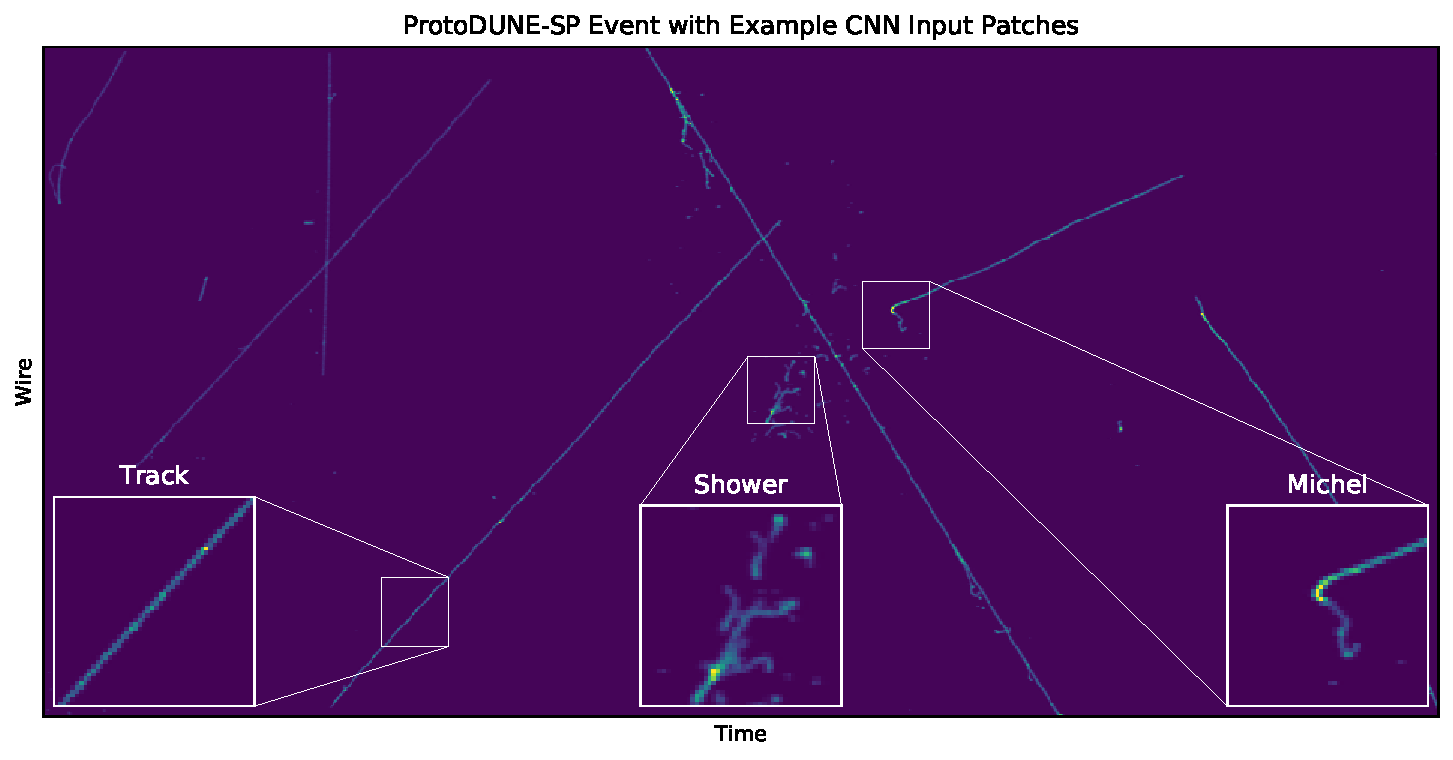
\includegraphics[width=\textwidth]{figures/patch_zoom.pdf}  
	\caption
	[Example CNN input images for each class.]
	{Example CNN input images for each class. The input images are $48 \times 48$
	pixel images, which are taken from regions of the full detector readout. In
	the diagram, one example of each image class is displayed. The white outlines
	demonstrate the location of each input image in the full readout.}
	\label{fig:patches}
\end{figure}

The true classification for each sample was obtained from the simulation, by 
associating the measured ionisation energy depositions to the corresponding
simulated particle. If the reconstructed hit is not associated to a true
particle, then this hit is due to noise and the true classification is empty.
Additional images were produced in empty regions of the detector, in the 
vicinity of charged particles, to increase the training sample for the empty 
category. The truth vectors for different true particle sources are detailed 
in Table \ref{tab:ground_truth}. These values were chosen based on the typical 
interaction type in \protodune{} for these particle species, which is based on 
the electromagnetic energy loss in liquid argon for energies in the GeV range.
\begin{table}
	\centering
	\bgroup
	\def\arraystretch{1.5}
	\begin{tabular}{c|c|c}
		Ionisation Source & Track, shower, empty & Michel \\ \hline
		Muons             & [1,0,0]              & [0]    \\
		Hadrons           & [1,0,0]              & [0]    \\
		Michel Electrons  & [0,1,0]              & [1]    \\
		Other Electrons   & [0,1,0]              & [0]    \\
		Noise             & [0,0,1]              & [0]    \\
	\end{tabular}
	\egroup
	\caption
	[Truth labels for the CNN output for different particle species.]
	{Truth labels for the CNN output for different particle species.}
	\label{tab:ground_truth}
\end{table}

The training data for the CNN was built using simulations of the \protodune{}
detector in the LArSoft framework; the simulations used were under beam
operating conditions and, therefore, included simulations of cosmic--rays, and
test beam particles in the range of 1--7 GeV. Around 29 million input images
were produced in total for the training. This sample was split into three
datasets, the training, validation, and test sets. The training set is used to
train the CNN, the validation set is used to monitor the performance of the CNN
during training, and the test set is used as an initial verification of the 
performance of the network after training. Details of the number of patches of
each type in these three datasets are detailed in Table \ref{tab:patches}.

\begin{table}
	\centering
	\bgroup
	\def\arraystretch{1.5}
	\begin{tabularx}{\textwidth}{@{}c|Y|Y|Y|Y|Y@{}}
		Dataset    & Shower     & Track      & Empty     & Michel  & Total      \\ \hline
		Training   & 13,493,982 & 9,727,604  & 2,517,882 & 731,456 & 26,470,925 \\
		Validation & 734,673    & 562,038    & 141,388   & 42,727  & 1,480,826  \\
		Test       & 764,659    & 518,805    & 139,987   & 39,674  & 1,463,125  \\ \hline
		Total      & 14,993,314 & 10,808,447 & 2,799,257 & 813,857 & 29,414,876
	\end{tabularx}
	\egroup
	\caption
	[Number of input images with each truth label.]
	{Number of input images with each truth label in the training, validation, and
	test sets.}
	\label{tab:patches}
\end{table}

\subsection{Network Architecture}

The network architecture for this CNN was designed to provide the best possible
performance given constraints on running time and memory usage during network
evaluation. This CNN is run on CPUs as part of the low level reconstruction 
chain for \protodune{}, and it's run time is required to be on the order of 10 
seconds per event. In addition, the CNN should not increase the maximum memory 
usage during reconstruction beyond around 4 GB. There is currently ongoing 
work looking into using GPUs during the network evaluation, which would decrease
the evaluation time, and allow more complex architectures to be used. 
Therefore, there is potential to increase performance of the method in the 
future.

The network architecture used is shown in Figure \ref{fig:arch}. The images
are first processed by convolutional layer with 48 $5 \times 5$ filters, this
layer extracts feature maps from the data. The responses from the 
convolutional layer are passed through the Leaky ReLU activation function, which
is discussed in Chapter \ref{ch:ml}, before being processed by the dense 
layers. The feature maps are processed by a pair of dense layers, with 128 and 
32 nodes respectively. These layers also use the Leaky ReLU activation
function. After the second dense layer the network is split into two branches in
order to make it's prediction. The first branch returns the prediction for the 
TSE categories, and the second branch for the Michel electron category. The 
first branch uses a Softmax activation function, which ensures that the scores 
for the TSE categories sum to one.  The second branch uses a Sigmoid 
activation function, which ensures that the Michel electron scores are bounded 
between zero and one. The choice of activation functions in the output layers 
allows for a pseudo--probabilistic interpretation of the scores from the CNN.

\begin{figure}
	\centering
	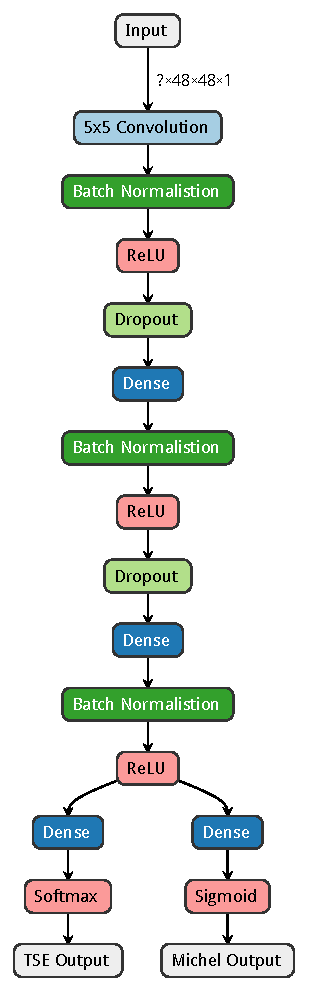
\includegraphics[height=0.9\textheight]{figures/track_shower_arch.pdf}
	\caption
	[Network architecture used for hit classification.]
	{Network architecture used for hit classification. Visualisation adapted from
	the Netron neural network viewer\cite{netron}.}
	\label{fig:arch}
\end{figure}

Two dropout layers are used in the network, these layers are used as part of the
regularisation of the network. A dropout probability of 0.5 is used in both of
the dropout layers. The dropout algorithm is discussed in Chapter \ref{ch:ml}.

The loss of the network was the weighted sum of the losses for the two output
branches,
\begin{equation*}
	L = 0.1 \cdot L_{TSE} + L_M,
\end{equation*}
where the Michel electron loss is given higher precedence due to the smaller
training dataset available for the Michel electron output. The loss function for
the TSE branch is the categorical cross entropy 
loss\cite{750fabedbacb467c8fafd98b87f77436}, and for the Michel electron branch
it is the mean squared error\cite{mse_springer},
\begin{align*}
	L_{TSE} &= - \frac{1}{N} \sum_{j=1}^N \sum_{i=0}^2 (t_j)_i \log (p_j)_i, \\
	L_M &= \frac{1}{N} \sum_{j=1}^N (t_j - p_j)^2
\end{align*}
where $t_j$ and $p_j$ are the truth and the prediction for the $j^{th}$ sample 
in the training batch, and $i$ sums over all outputs in the TSE branch. 

\subsection{Training and Validation}
The TensorFlow\cite{45381} library and the Keras\cite{chollet2015keras} 
application programming interface (API) were used to design and train the CNN. 
The training was completed on a dedicated \protodune{} server at CERN, with an 
NVIDIA GTX 1080 GPU. Training was monitored using the TensorBoard visualisation 
toolkit\cite{tensorboard}, which is part of the TensorFlow library. 

The CNN was trained using the mini--batch stochastic gradient descent (SGD)
algorithm, including both the momentum and decay algorithms\cite{Reed1999}. 
The momentum algorithm reduces the oscillations of the weights during 
learning, while the decay of the learning rate allows for rapid learning 
during early stages of SGD, and increased precision as the model converges. 

During training the learning metrics where monitored with TensorBoard. The
losses for each branch and the total loss were monitored for the training
and validation datasets. The validation loss was calculated once per training
epoch, which is one iteration through the full training dataset, and the
training loss is averaged at the end of each epoch. The training and validation
losses as a function of training epoch are shown in Figure \ref{fig:training}.
The weights of the network were saved at the end of each epoch. The final
weights were chosen based on the early stopping algorithm discussed in Chapter
\ref{ch:ml}, focussing on the TSE branch of the network, this is highlighted 
in Figure \ref{fig:training}.
\begin{figure}
	\centering
	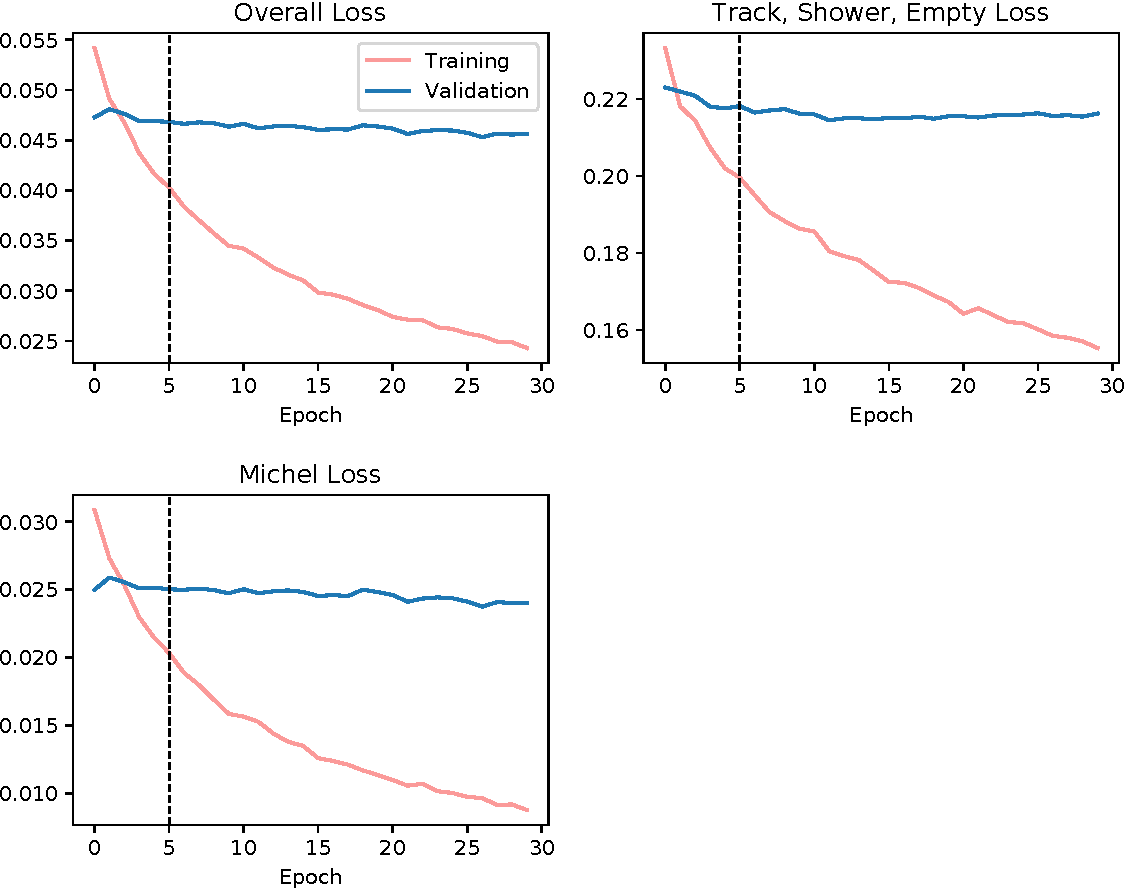
\includegraphics[width=\textwidth]{figures/losses_prelu.pdf}
	\caption
	[Evolution of the validation and training set losses during the training 
	process.]
	{Evolution of the validation and training set losses during the training 
	process. The losses for the TSE branch and the Michel electron branch are
	shown, as well as the total loss. The weights were frozen based on an early 
	stopping algorithm, focussing on the loss in the TSE branch. The losses with
	the weights chosen by the early stopping algorithm are indicated by a vertical
	dashed line on each diagram.} 
	\label{fig:training}
\end{figure}

During training, the validation loss remains stable over a number of epochs,
which suggests that the dropout algorithm was successful in preventing 
over--fitting. After training, the networks performance was verified against 
the test set, which found that the test set losses were compatible with the 
validation set loss. The final test set losses were, 
\begin{align*}
	L &       = 0.033, \\
	L_{TSE} & = 0.155, \\
	L_M &     = 0.017.
\end{align*}

\section{Performance on ProtoDUNE--SP Simulation} \label{cnn-perf-sim}

The performance of the hit tagging algorithm was evaluated with reconstructed
events from \protodune{} simulation, the dataset used for this performance
analysis was distinct from the training, validation, and test sets. 

The distributions of the shower score from the TSE classifier for true shower 
hits and all other hits is given in Figure \ref{fig:show_output}. There is a 
strong separation seen between the distributions for the shower and track 
hits, showing that the network has strong discriminating power. In practice, the
empty score of the TSE classifier was found to be on the order of $10^{-9}$ or
smaller for all hits tested. As such,
\begin{equation*}
	\mbox{TrackScore} \approx 1 - \mbox{ShowerScore},
\end{equation*}
which means that the results of the analysis of the shower score are valid for
the analysis of the track score. Therefore, we will only discuss the shower
score from now on.

The shower classification threshold for subsequent algorithms should be tuned on
a case by case basis, however, for this study a simple optimisation strategy 
is presented in order to quantify the basic network performance. This is based
on the $F_1$ metric, a specific case of the $F_\beta$ 
metric\cite{VanRijsbergenC.J.1975Ir}, which places equal importance on 
precision and recall. The $F_1$ metric is given by, 
\begin{equation*}
	\frac{1}{F_1} = \frac{1}{\mbox{precision}} + \frac{1}{\mbox{recall}},
\end{equation*}
where we define the precision as the fraction of correctly classified shower 
hits in the sample of all selected shower hits, and the recall as the fraction 
of all true shower hits, which were selected as shower hits. The $F_1$ score 
was calculated across a range of selection thresholds, this is shown in Figure 
\ref{fig:show_output}. The score peaks at a threshold of 0.72 where,
\begin{equation*}
	F_1 = \mbox{precision} = \mbox{recall} = 0.863.
\end{equation*}

\begin{figure}
	\centering
	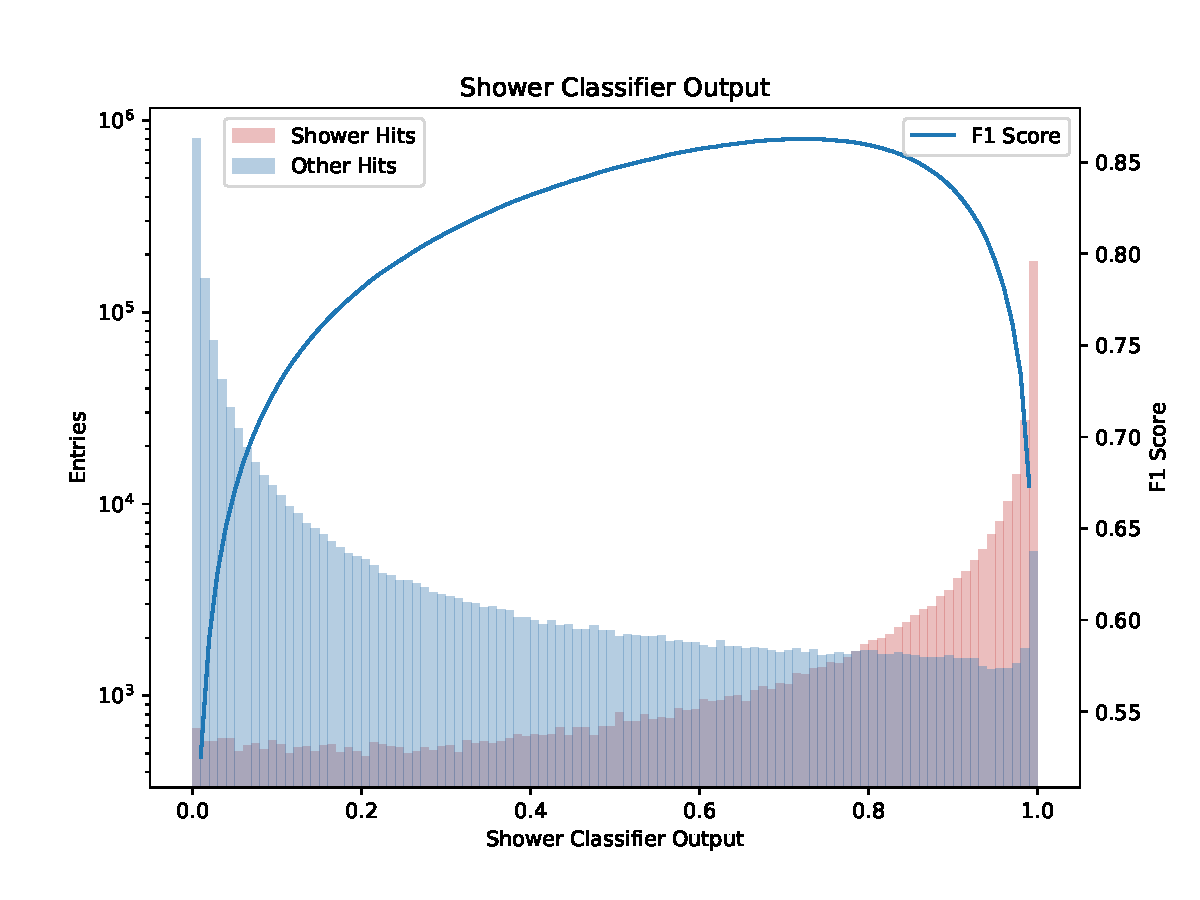
\includegraphics[width=0.9\textwidth]{figures/shower_combined.pdf} 
	\caption
	[Shower score output distributions for the TSE classifier.]
	{Shower score output distributions for the TSE classifier. The score
	distributions for true shower hits and all other hits are shown in red and
	blue respectively. Threshold optimisation was done using the F1 score metric, 
	which is also plotted as a function of the classification threshold.}
	\label{fig:show_output}
\end{figure}

The overall performance of the TSE classifier can also be evaluated with a
receiver operating characteristic (ROC) curve\cite{Fawcett2006}. The ROC curve
shows the true--positive rate vs the false--positive rate for the classifier, as
the selection threshold is varied. Figure \ref{fig:show_roc} shows two ROC
curves for the TSE classifier, one is evaluated in simulation including
the space charge effect (SCE), and the other excludes the SCE. Both curves
demonstrate that the network is capable of achieving high true--positive rates,
while maintaining low false--positive rates. In addition, their is a very close
agreement between the two curves, which suggests that the TSE classifier is
robust to changes in the SCE model.

\begin{figure}
	\centering
	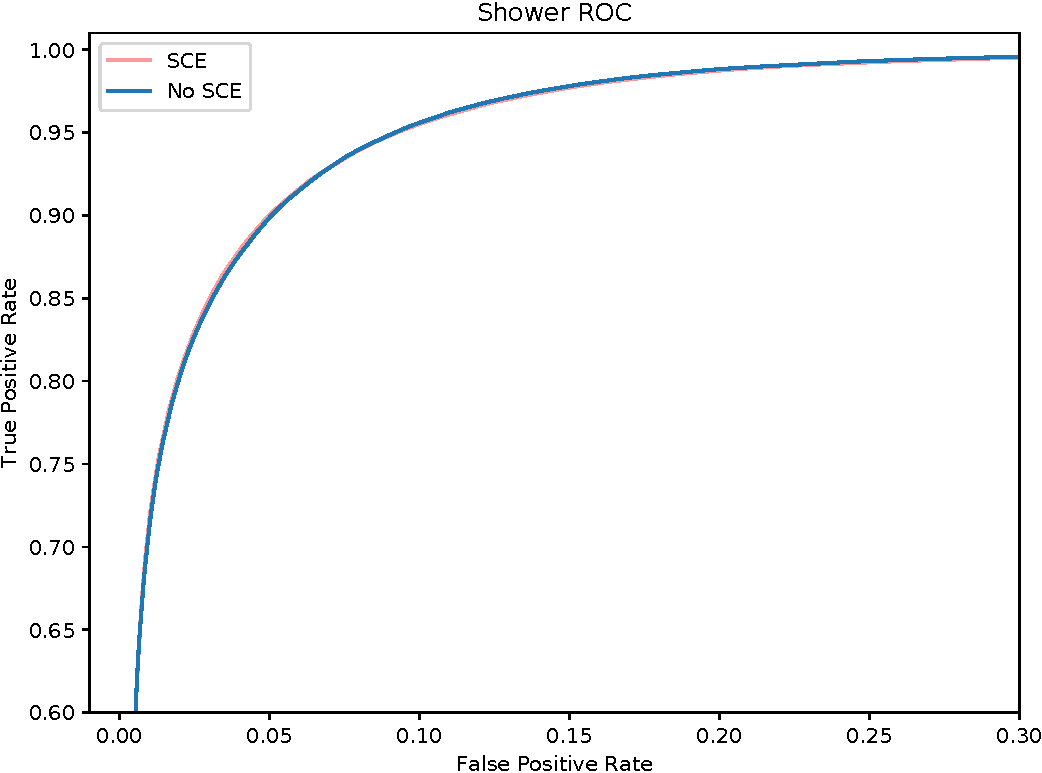
\includegraphics[width=0.9\textwidth]{figures/show_roc_comparison.pdf}
	\caption
	[ROC curves for the shower score from the TSE classifier.]
	{ROC curves for the shower score from the TSE classifier. These curves show
	the true--positive rate vs the false--positive rate for varying classification
	thresholds. The ROC curves for the \protodune{} simulation including SCE and
	excluding SCE are shown in red and blue respectively. The ROC curve in the
	presence of SCE is concealed by the curve without SCE.}
	\label{fig:show_roc}
\end{figure}

The performance of the Michel electron classifier was analysed with the same
methods as the shower classifier. The Michel electron score distribution for
true Michel electron hits and all other hits is shown in Figure
\ref{fig:michel_output}. In this case the large discrepancy in sample size
between Michel electron hits and other hits, leads to a low F1 score of around
0.2 when considering the performance on a hit--by--hit basis. However, in
Chapter \ref{ch:michel}, we will see that despite the low performance of the
classifier for individual hits, a pure sample of Michel electron events can be
selected by searching for clusters of hits with high Michel electron scores.

\begin{figure}
	\centering
	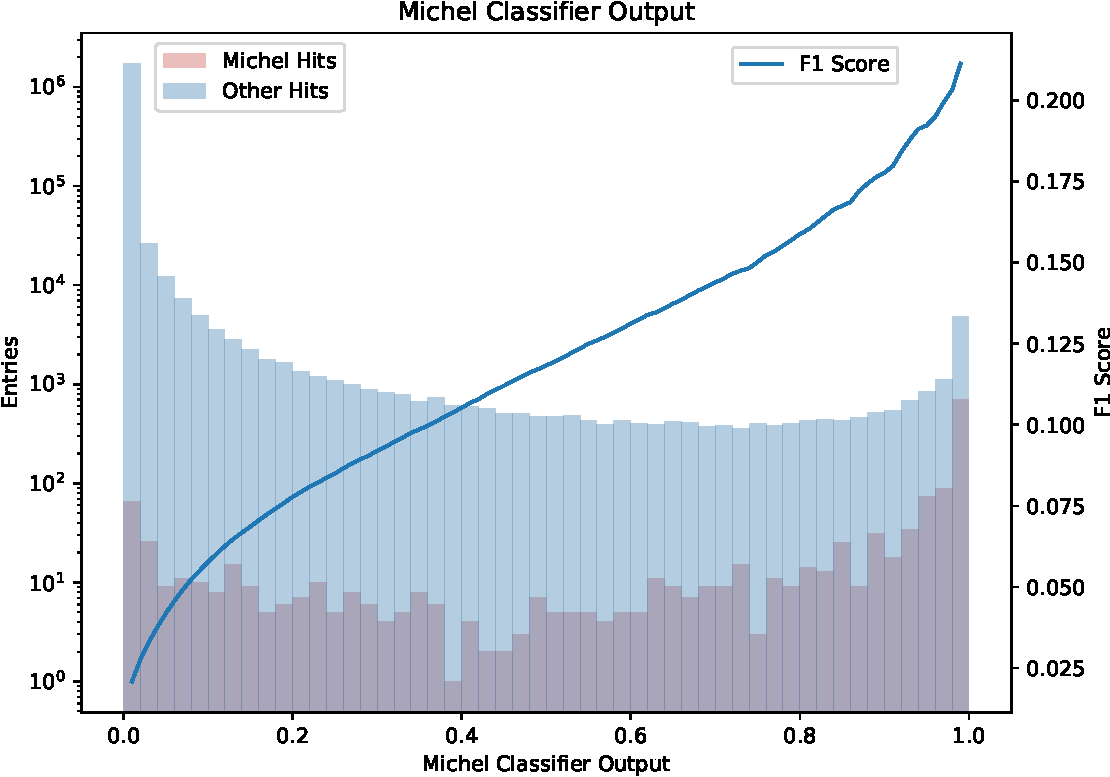
\includegraphics[width=0.9\textwidth]{figures/michel_combined.pdf} 
	\caption
	[Michel electron score distributions for the Michel electron classifier.]
	{Michel electron score distributions for the Michel electron classifier. The
	score distributions for true Michel electron hits and all other hits are shown
	in red and blue respectively. The F1 score metric was used to assist 
	threshold selection, and is also plotted as a function of selection 
	threshold. The final threshold was modified when combined with a clustering 
	algorithm, see the analysis in Chapter \ref{ch:michel}.}
	\label{fig:michel_output}
\end{figure}

The ROC curve is independent of the relevant size of each true sample and,
therefore, it provides a more instructive evaluation of the performance of the
Michel electron classifier than the score distribution and F1 score. The ROC 
curves for the Michel electron classifier are shown in Figure 
\ref{fig:michel_roc}, where both SCE and no SCE samples are shown. The jitter 
in the lines is due to the smaller sample size in this case. In both cases the 
Michel electron classifier is able to achieve a true--positive rate of over 90\%,
while maintaining a false--positive rate of less than 2.5\%. There is a larger 
difference between the SCE and no SCE curves for the Michel electron sample,
however, the difference is still no bigger than 4\%.

\begin{figure}
	\centering
	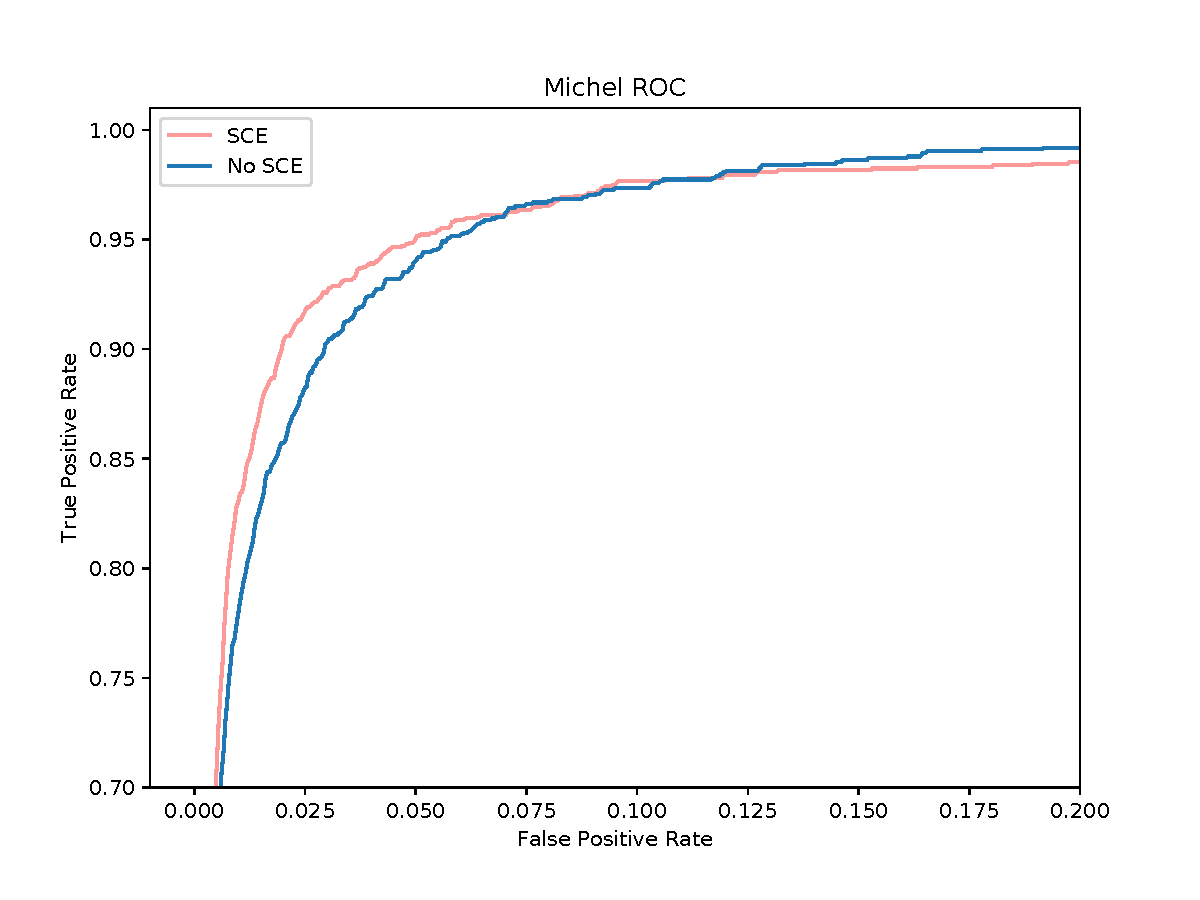
\includegraphics[width=0.9\textwidth]{figures/michel_roc_comparison.pdf}
	\caption
	[ROC curves for the Michel electron classifier.]
	{ROC curves for the Michel electron classifier. These curves show
	the true--positive rate vs the false--positive rate for varying classification
	thresholds. The ROC curves for the \protodune{} simulation including SCE and
	excluding SCE are shown in red and blue respectively.}
	\label{fig:michel_roc}
\end{figure}

\subsection{Comparison with Pandora}
Pandora is the primary reconstruction framework used in \protodune{}, it was
discussed in Chapter \ref{ch:protodune}. One of the goals of the CNN is to
provide supplementary information to Pandora, to assist analysers in defining 
pure event samples. This is possible because Pandora and the CNN have slightly
different goals, Pandora aims to cluster hits in the most appropriate way based
on their spatial distribution, while the CNN aims to classify the hits based on 
the particle that caused the energy deposition.

The comparison of the particle classification to Pandora was done with a beam 
particle sample in \protodune{} simulation, including the primary particle and 
any daughters. The true particle type was obtained from the simulation, and 
the track--shower categorisation was compared between Pandora and the CNN. For 
Pandora, the type of reconstructed cluster was taken as the classification. 
For the CNN the average shower score for the hits in the particle was 
calculated and compared to a threshold of 0.72, based on the previous F1 score 
calculation. Any particles with an average shower score above the threshold were
classified as showers, and any with score below the threshold were classified 
as tracks. 

The particle classification by particle species based on the Pandora method and
the CNN method are compared in Figure \ref{fig:track_show_pan_cnn}, which 
shows the fraction of each particle species classified as tracks and showers 
by Pandora and the CNN. We can see that CNN gives a stronger classification 
than Pandora for all particle species. Electron and photons are more often 
classified as showers, and pions, muons, and protons are more often classified 
as tracks. 
\begin{figure}
	\centering
	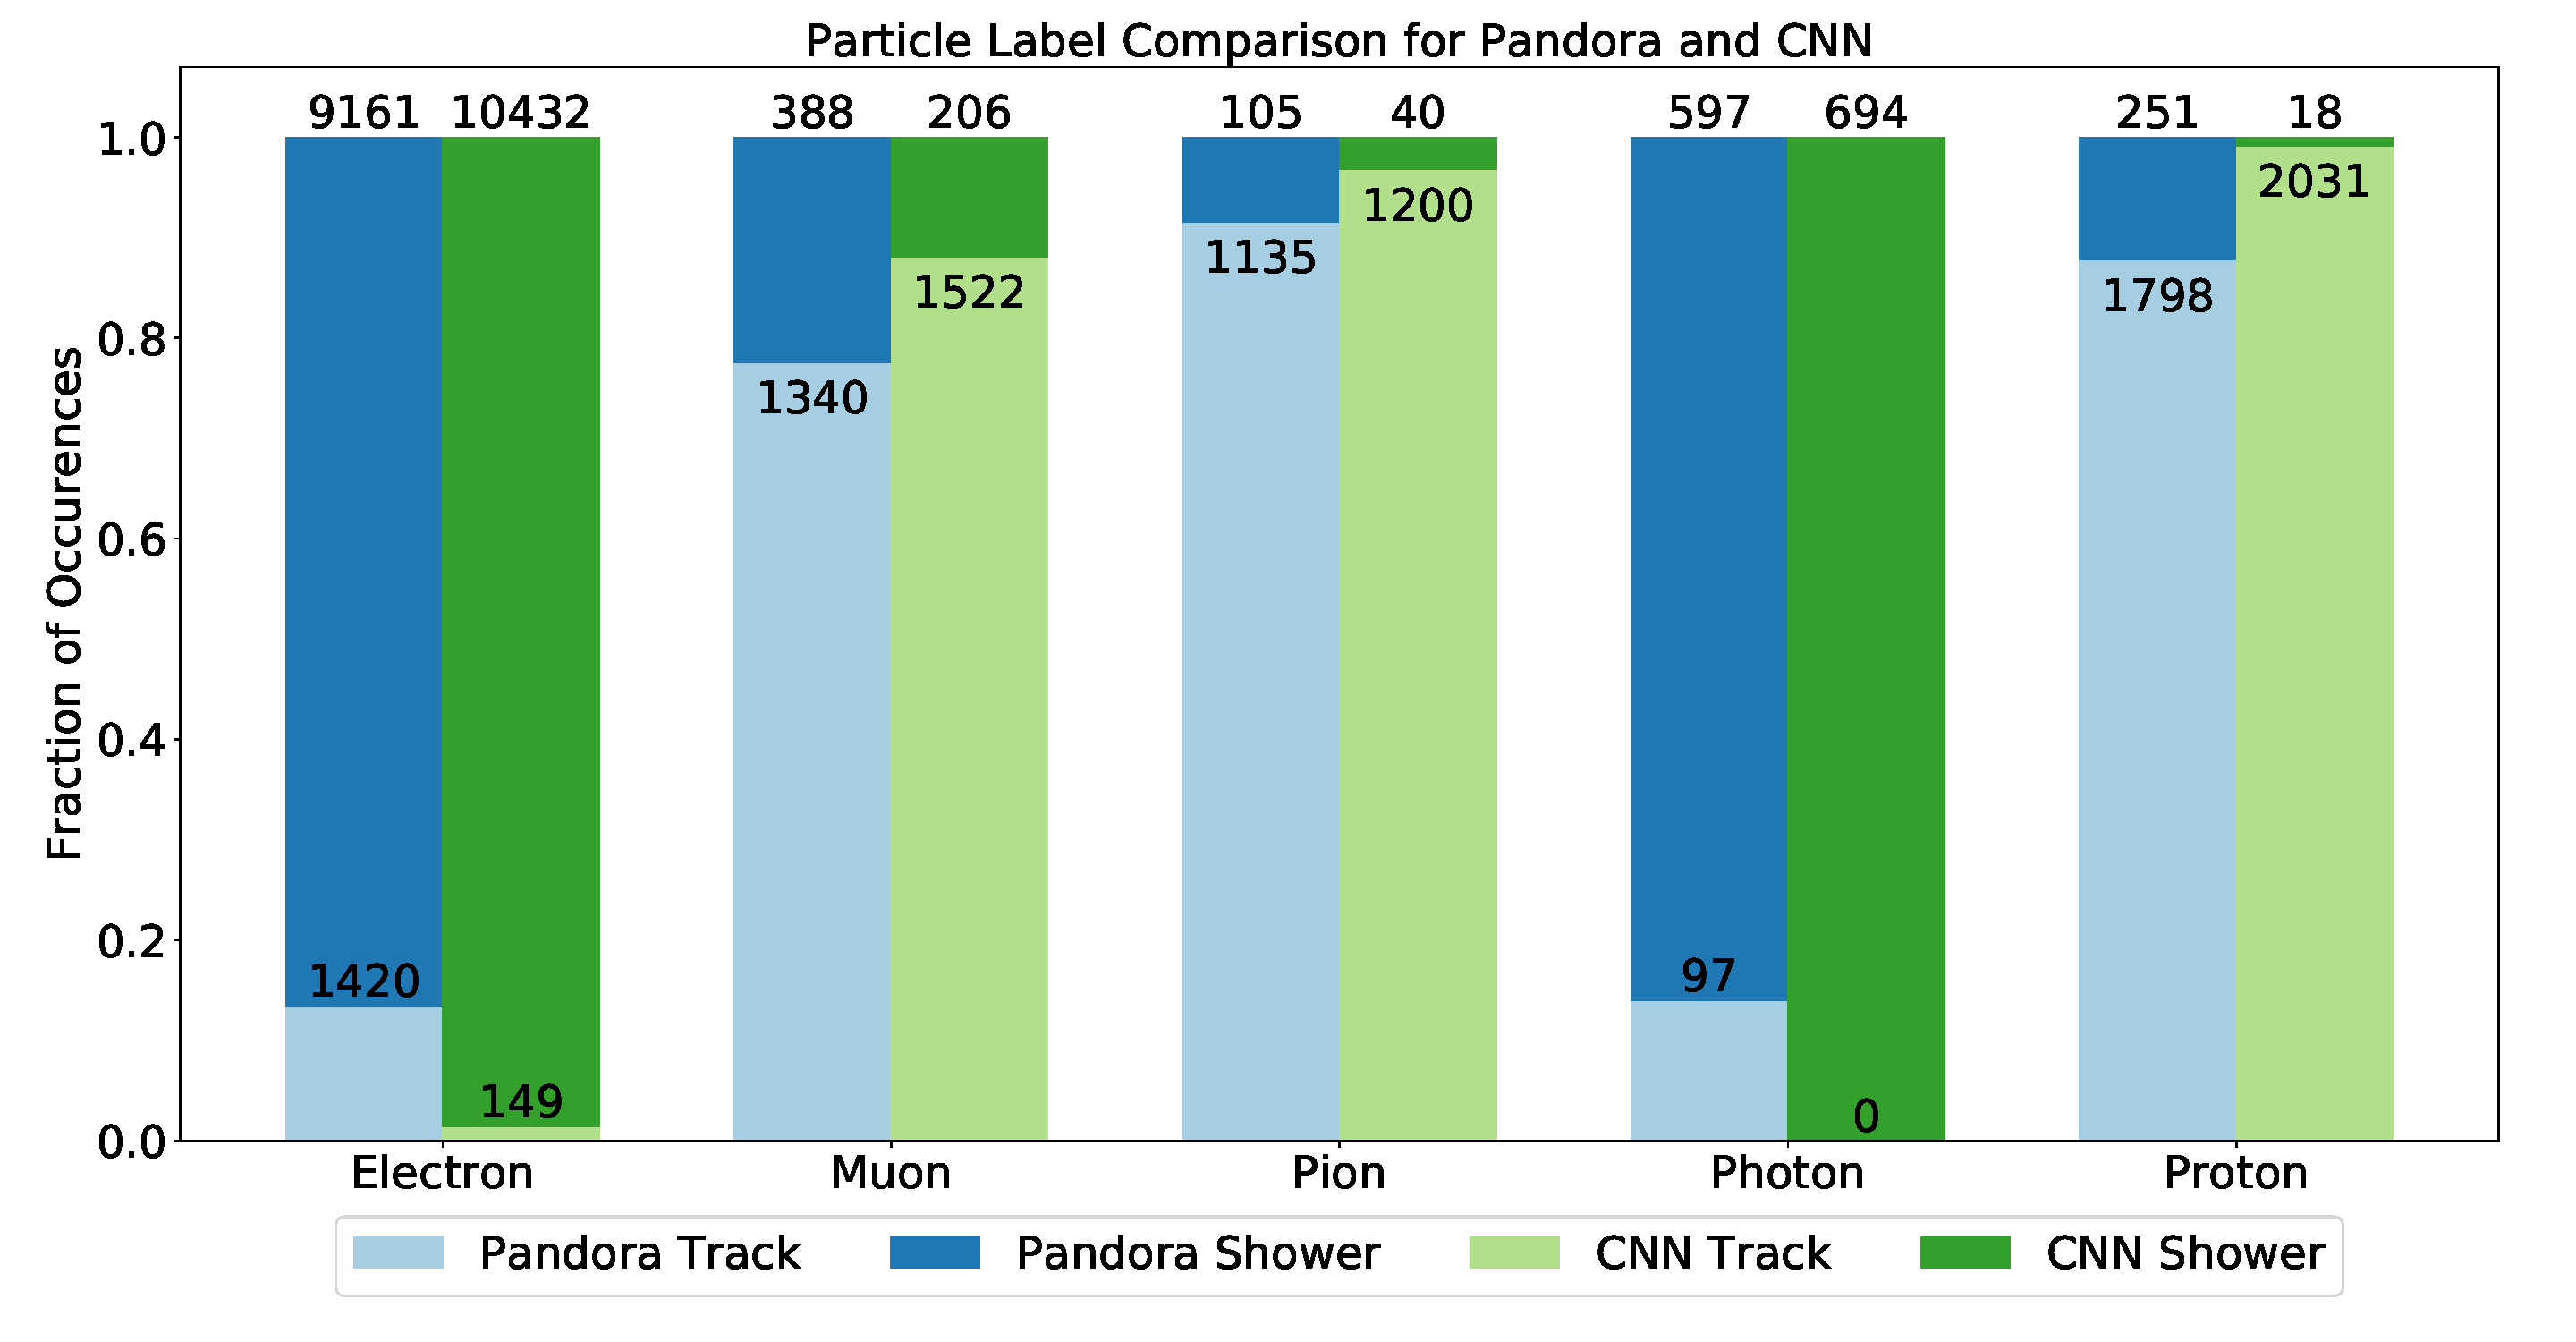
\includegraphics[width=\textwidth]{figures/track_shower_labels.pdf}
	\caption
	[Comparison of track and shower classifications by Pandora and the CNN.]
	{Comparison of track and shower classifications by Pandora and the CNN. For
	each true particle species the fraction of events classified as tracks and
	showers is shown, for Pandora and the CNN. Each bar is labelled with the 
	number of events, for example, the CNN classified 149 electron events as 
	tracks and 10432 electron events as showers.}
	\label{fig:track_show_pan_cnn}
\end{figure}

The false--positive rates (FPR) for Pandora and the CNN for each particle 
species are given in Table \ref{tab:false_pos}, as well as their ratio.
The CNN only gives a modest improvement over Pandora for pions, and muons. 
However, there is a significant improvement in the false--positive rate for 
electrons, photons, and protons. The biggest improvement is for photons, 
where for a sample of 694 photons, the CNN has a false--positive rate of zero.
\begin{table}
	\centering
	\bgroup 
	\def\arraystretch{1.5}
	\begin{tabularx}{\textwidth}{@{}c|Y|Y|Y|Y|Y@{}}
		Particle Species & Electron & Photon & Muon  & Pion  & Proton \\\hline
		Sample Size      & 10,581   & 694    & 1,728 & 1,240 & 2,049  \\\hline
		Pandora FPR (\%) & 13.4     & 13.9   & 22.5  & 8.5   & 12.2   \\
		CNN FPR (\%)     & 1.4      & 0.0    & 11.9  & 3.2   & 0.9    \\\hline
		Pandora / CNN    & 9.53     & --     & 1.88  & 2.62  & 13.9   \\
	\end{tabularx}
	\egroup
	\caption
	[False--positive rates for track shower classification with Pandora and the
	CNN.]
	{False--positive rates for track shower classification with Pandora and the
	CNN. The false--positive rates for both the CNN and Pandora are given for
	different particle species. In addition, the sample size for each particle
	species, and the ratio of the false positive rate of Pandora to the 
	CNN are given whenever possible.}
	\label{tab:false_pos}
\end{table}

The stronger classification from the CNN gives supplementary information to
Pandora, which can be used in analyses to improve event selection or background
rejection. This information is being utilised in a number of \protodune{}
analyses, some of these analyses are highlighted briefly in Section
\ref{cnn-appl}.

As well as providing supplementary information to Pandora for analysis, the CNN
scores could be utilised during Pandora reconstruction as an additional guide
for the reconstruction algorithms. This approach is being developed by Pandora
for the DUNE far detector, based on a similar deep neural network for 
discriminating tracks and showers\cite{chappel_poster}.

\section{Validation on \protodune{} Data} \label{cnn-perf-data}

For validation on real \protodune{} data three approaches were used: visual
validation with event scans, comparisons of the overall score distributions, 
and the comparison of score distributions for different particle species. Data 
from \protodune{} runs 5387 and 5809 were used for these validations; the data 
for these run was taken under stable operating conditions, with an average 
beam energy of 1 GeV. The beam composition in run 5387 was tuned to contain
mostly hadrons, while in run 5809 it was tuned to have an enhanced electron
component. The same operating conditions were used for the simulated data, in
order to give the closest possible comparison between data and simulation.

As discussed in Section \ref{cnn-perf-sim}, the sample of Michel electron hits
is orders of magnitude smaller than the other hits. In order to make a
meaningful validation of the performance of the Michel electron classifier on
data, the fraction of Michel electron hits in the sample needs to be increased.
Therefore, discussion of the validation of the Michel electron classifier will 
be postponed until Chapter \ref{ch:michel}, which will discuss Michel electron 
event selection and reconstruction.

Hand scans of the events show qualitatively that the performance on the data is
good. Figure \ref{fig:real_event} shows an example of the track score for hits
in a reconstructed event from run 5387. The hits in this image are from the
collection plane near the beam entry point, an electron shower tagged by the
beam instrumentation (BI) can be seen near the centre of the image. In the event
we can see that for hits in the tracks the CNN produces a large output score,
and for the shower like activity in the event the score is low, as we expect. In
addition, the classifier is able to identify that the hits adjacent to the 
track, which are from delta rays, are from electrons.

\begin{figure}
	\centering
	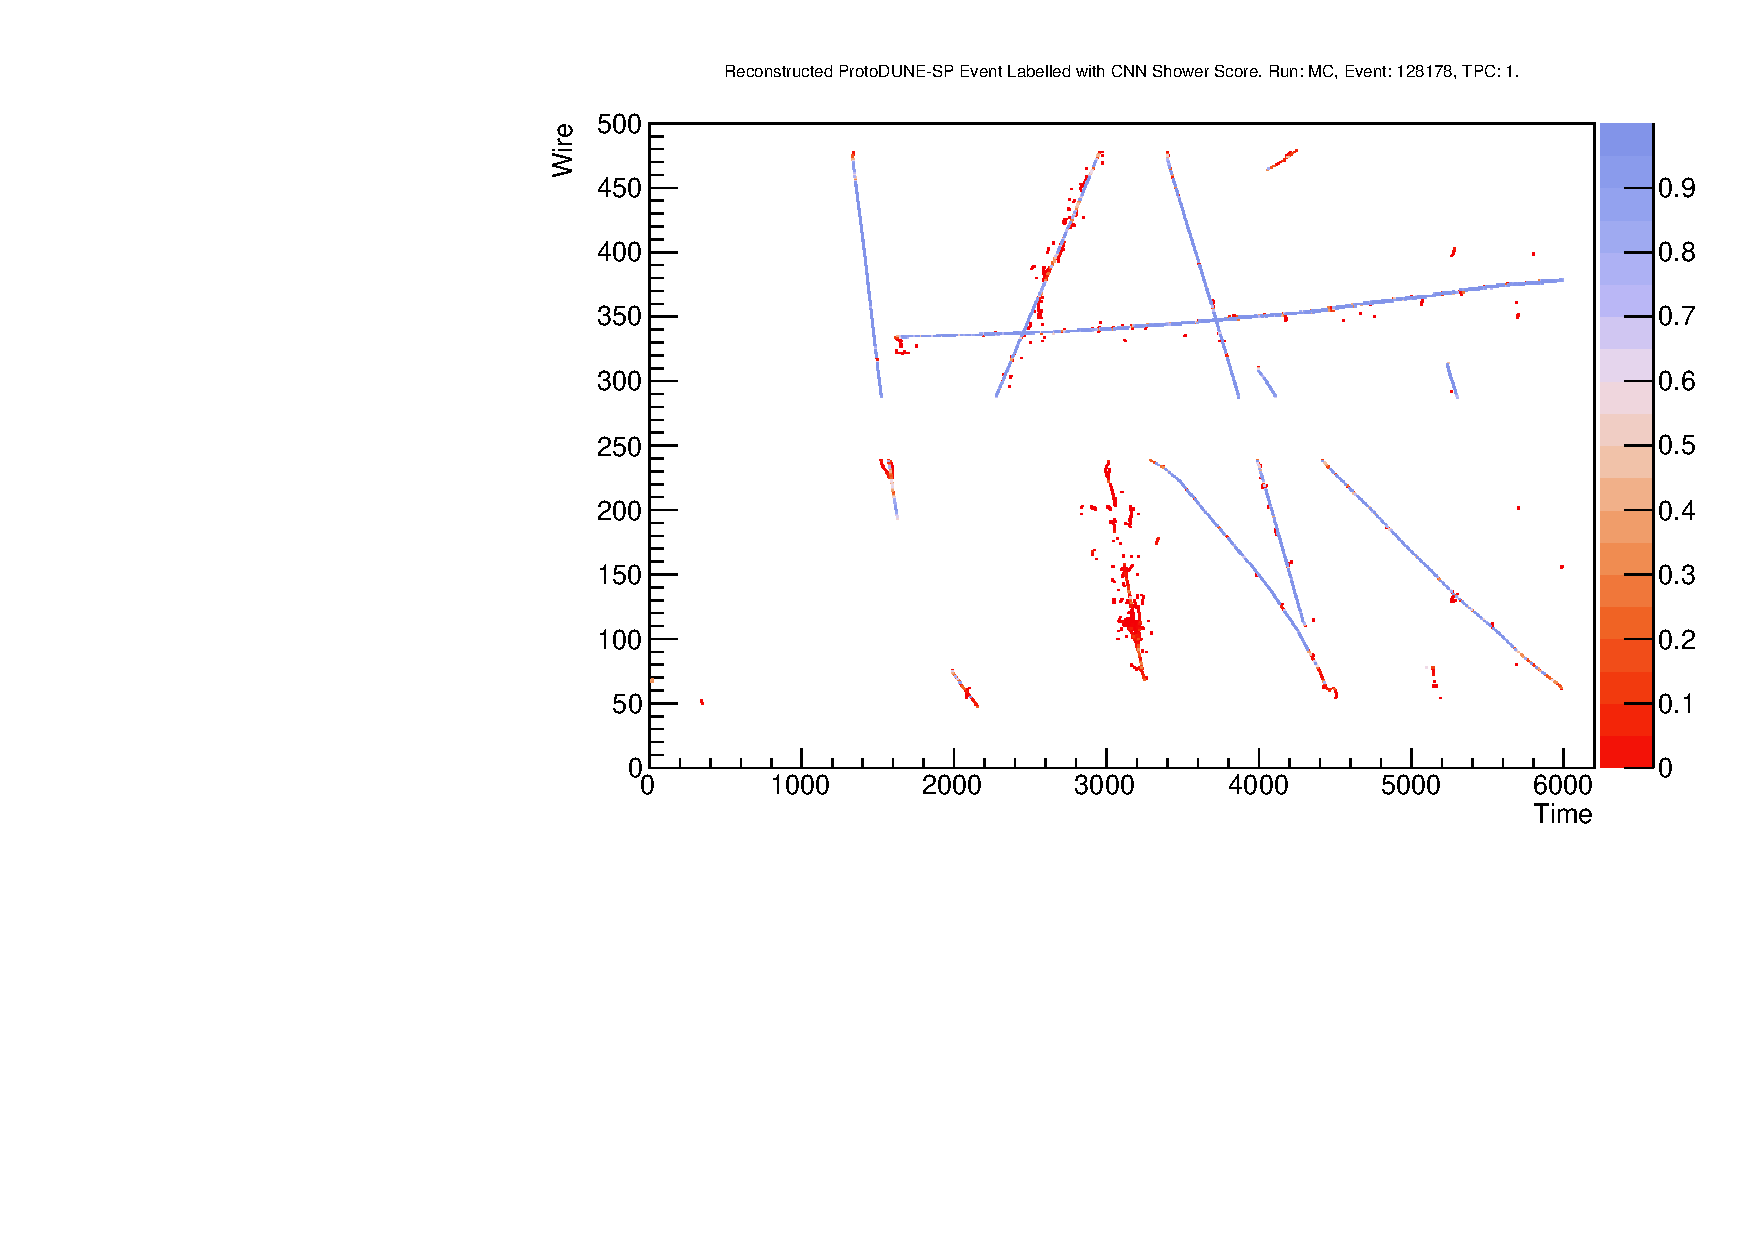
\includegraphics[width=\textwidth]{figures/5387_image_tpc1_view2_128178.pdf}
	\caption
	[Track classifier scores for a reconstructed event in \protodune{} data.]
	{Track classifier scores for a reconstructed event in \protodune{} data. Each
	reconstructed hit is labelled with its track classifier score, and located at
	the reconstructed wire and time coordinates.}
	\label{fig:real_event}
\end{figure}

The shower score distribution for all hits gives an overall validation of the 
network performance between data and simulation. It is the only quantitative 
validation method for the CNN, which remains decoupled from the Pandora 
reconstruction algorithm. Therefore, it is independent of the differences 
between data and simulation, which impact the results of Pandora.  The 
comparison is still dependent on the noise removal algorithm, the hit tagging 
algorithm, and the particle flux, which impact the input images to the CNN.

In this comparison, and the following beam particle comparisons, a cut is made 
on the reconstructed charge of each hit. This cuts out the excess of low 
charge hits in data, as illustrated in Figure \ref{fig:charge_cuts}.  In 
addition, all hits in the first 45 cm of the APA closest to the beam entry 
point were removed. This region has a known issue in charge simulation, which 
can be seen as a discontinuity in the reconstructed charge. This charge 
discontinuity can be seen in in Figure \ref{fig:90_wires_charge}, which 
demonstrates the discontinuity for a simulated proton beam sample.  

\begin{figure}

	\begin{subfigure}[b]{\textwidth}
		\centering
		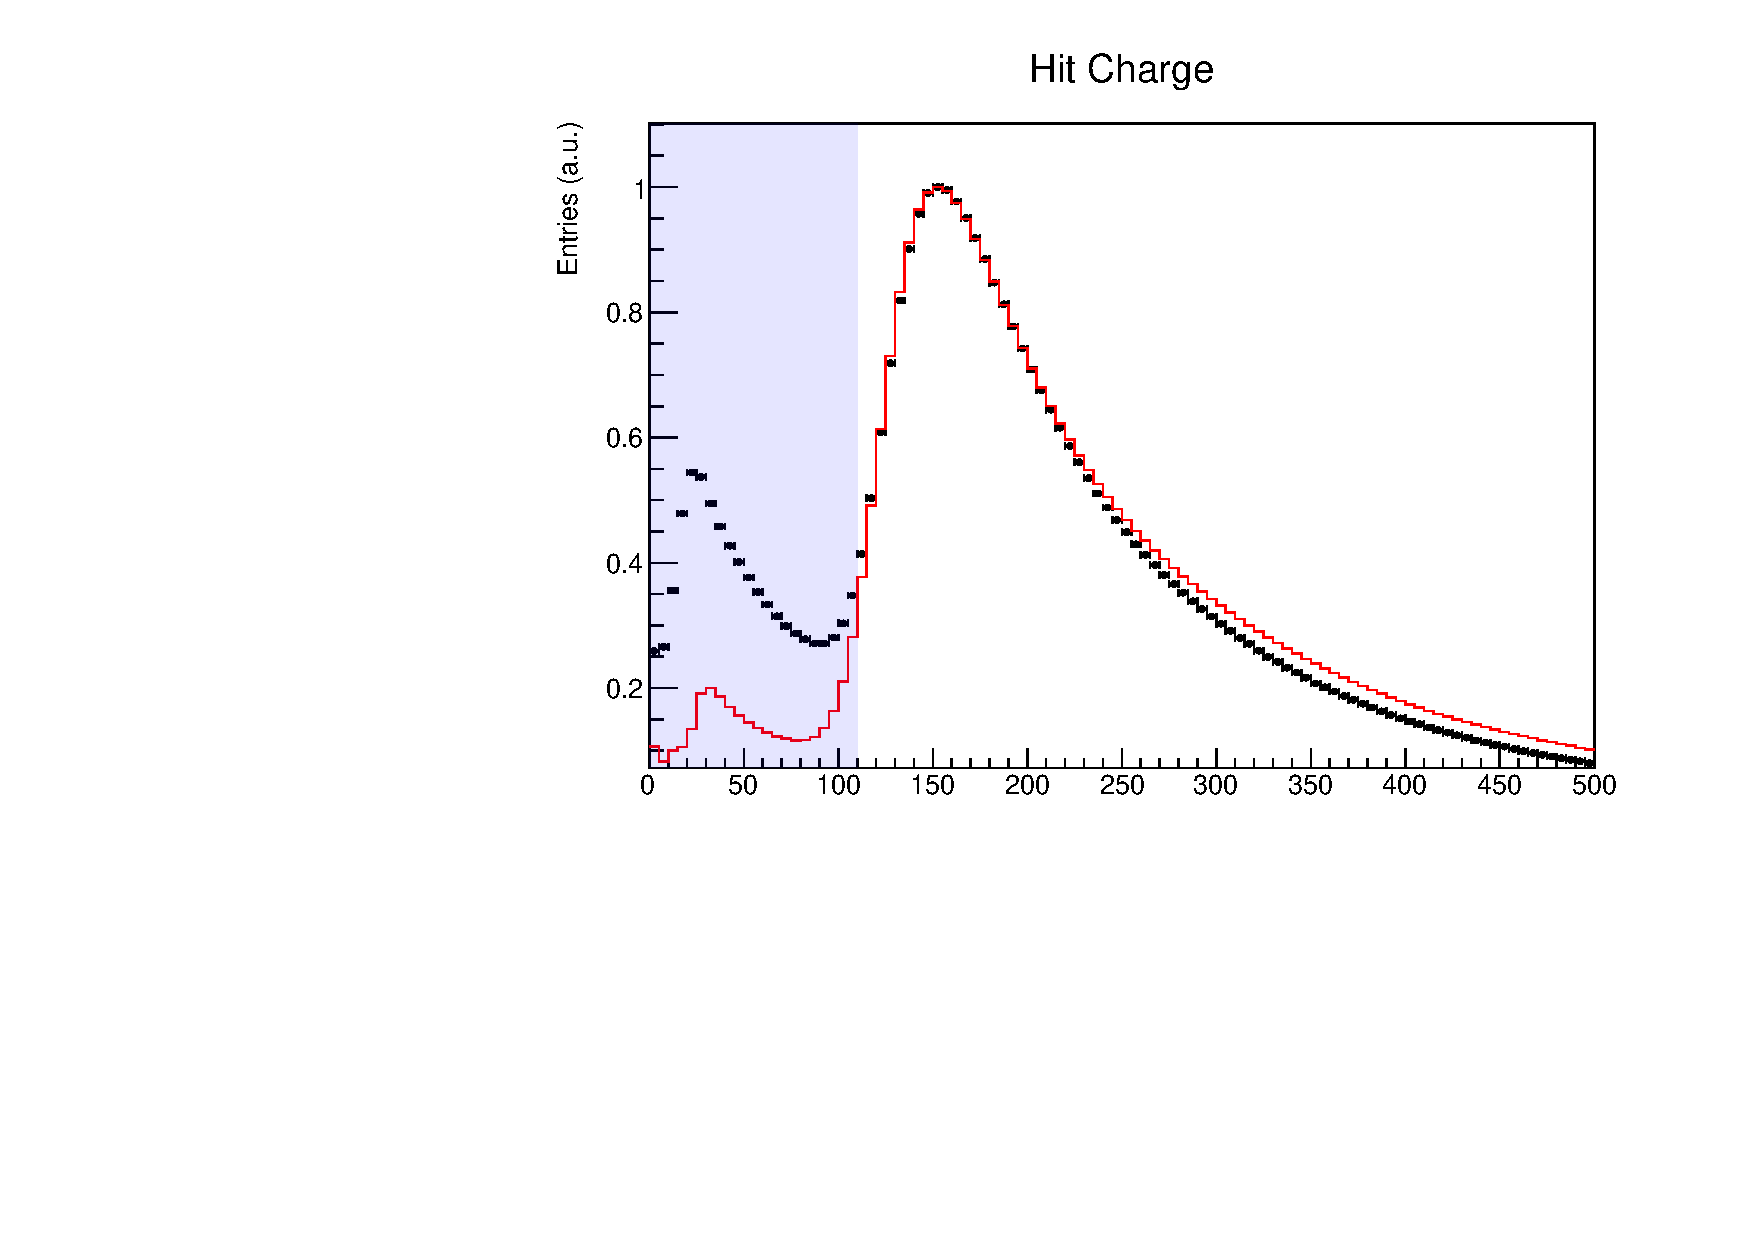
\includegraphics[width=0.8\textwidth]{figures/charge_nocuts.pdf}
		\caption {Cut on the reconstructed hit charge.}
		\label{fig:charge_cuts}
	\end{subfigure}

	\begin{subfigure}[b]{\textwidth}
		\centering
		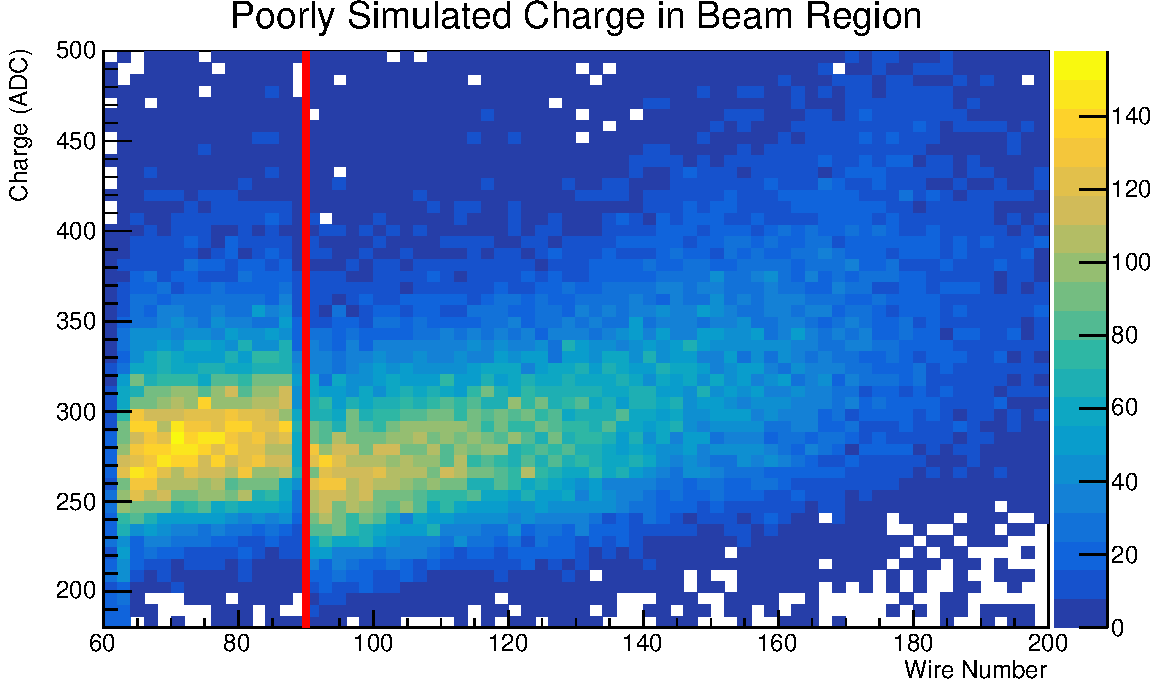
\includegraphics[width=0.8\textwidth]{figures/charge_discontinuity.pdf}
		\caption {Cut on the reconstructed wire, due to a charge discontinuity in
		simulation.}
		\label{fig:90_wires_charge}
	\end{subfigure}

	\caption 
	[ Quality cuts on reconstructed hits for CNN comparison. ]
	{ Quality cuts on reconstructed hits for CNN comparison. }
	\label{fig:cnn_cuts_charge}

\end{figure}

The overall shower score distribution for data and simulation is shown in 
Figure \ref{fig:cnn_overall_score}, as well as the fractional residuals in 
each bin. These distributions are normalised by the number of hits, allowing us
to compare the shape of the score distribution in data and simulation.  
Overall there is a good agreement between the data and the simulation, 
however, the distribution in data has a slightly different shape at low CNN
scores. This can be seen in the residuals, which have a negative slope for 
hits with shower score less than around 0.2.
\begin{figure}
	\centering
	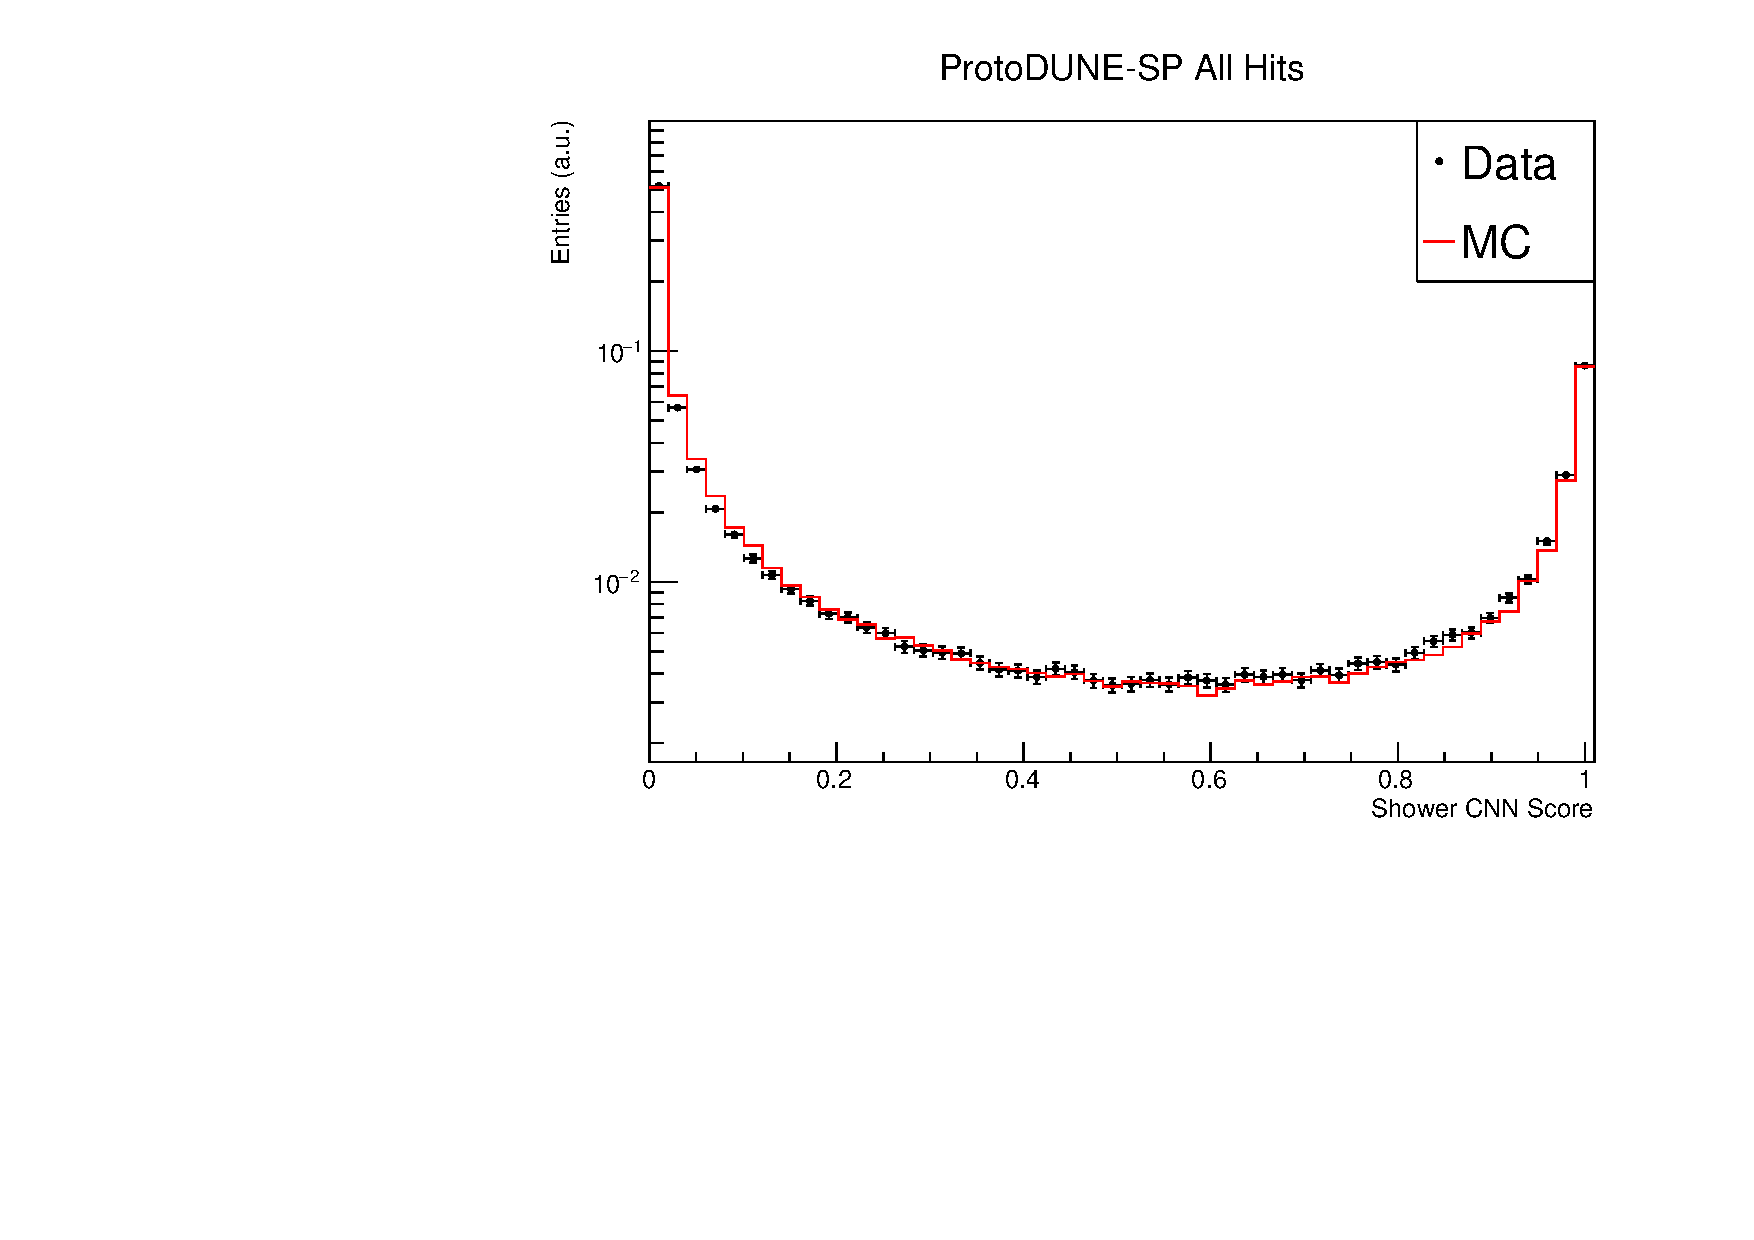
\includegraphics[width=\textwidth]{figures/hit_cnn_all.pdf}
	\caption
	[Overall shower score distribution from the CNN for all hits in data and simulation.]
	{Overall shower score distribution from the CNN for all hits in data and
	simulation. The top panel shows the shower score distribution for all hits in
	data and simulation, normalised by the number of hits. The fractional 
	residuals in each bin are shown in the bottom plot.}
	\label{fig:cnn_overall_score}
\end{figure}

We can also consider the comparison of the CNN to data for specific particle 
species, such as beam particles and cosmic--rays.  The BI in \protodune{} 
provides PID for beam particles with a very high purity. Therefore, in the 
case of particles originating from the charged particle beam, the BI can be 
used to provide an effective truth source. This allows the results of the CNN 
to be compared between data and simulation for different particle species. Any 
particles that arrive out--of--time with the beam can be assumed to be 
cosmic--rays and, therefore, form an additional truth source. The shower score 
distributions for electrons, pions, protons, and cosmic--rays are produced 
based on these samples. 

It is important to note that the results for these true particle 
samples rely on both Pandora and the CNN scores. Therefore, phase space cuts 
were made, to select regions of the detector where Pandora has a good 
agreement between data and simulation. The aim of these cuts was to to 
minimise the impact of Pandora on the observed CNN score distributions. Cuts 
on the start and end points of the reconstructed tracks were made, with the 
same cuts being applied to both the start and end point of each track. These 
cuts are illustrated for the end point of the tracks in Figure 
\ref{fig:spatial_cuts}.  The reconstructed angular distributions for tracks 
after these cuts are shown in Figure \ref{fig:angular_dist}.

\begin{figure}

	\begin{subfigure}[b]{\textwidth}
		\centering
		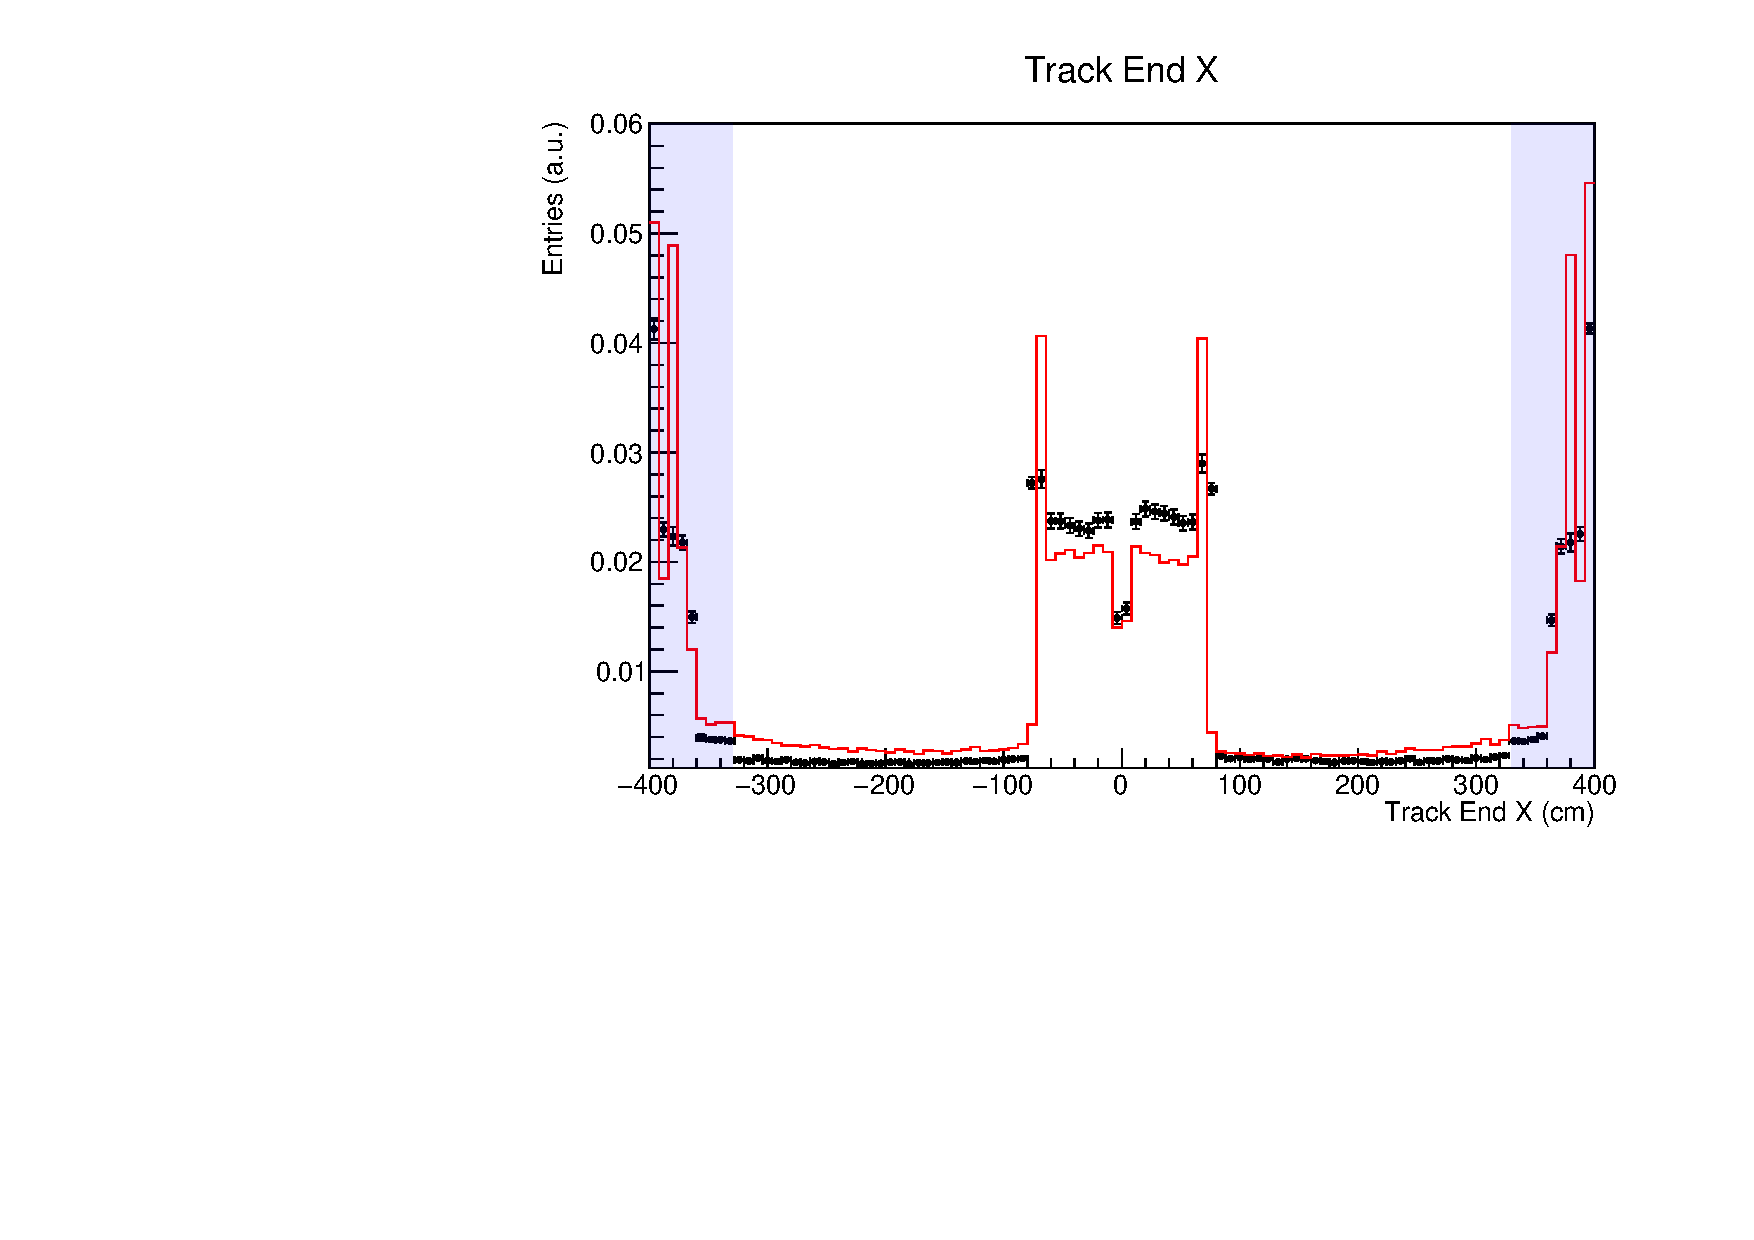
\includegraphics[width=0.49\textwidth]{figures/endX_nocuts.pdf}
		\hfill
		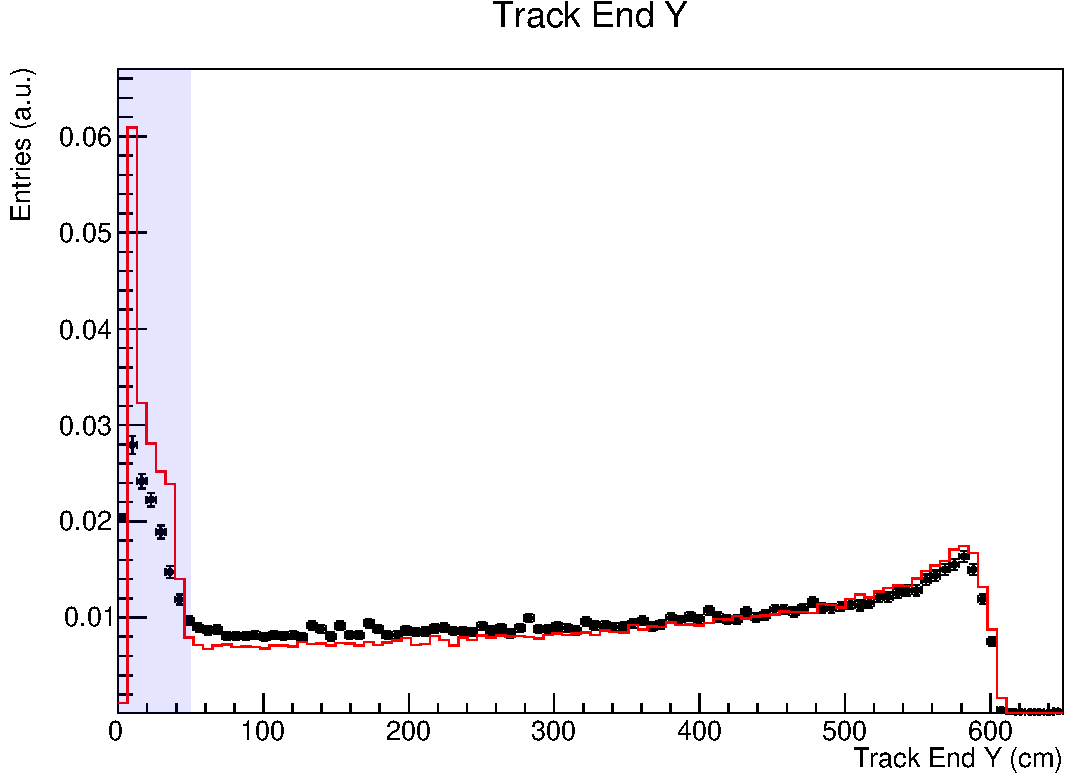
\includegraphics[width=0.49\textwidth]{figures/endY_nocuts.pdf}
		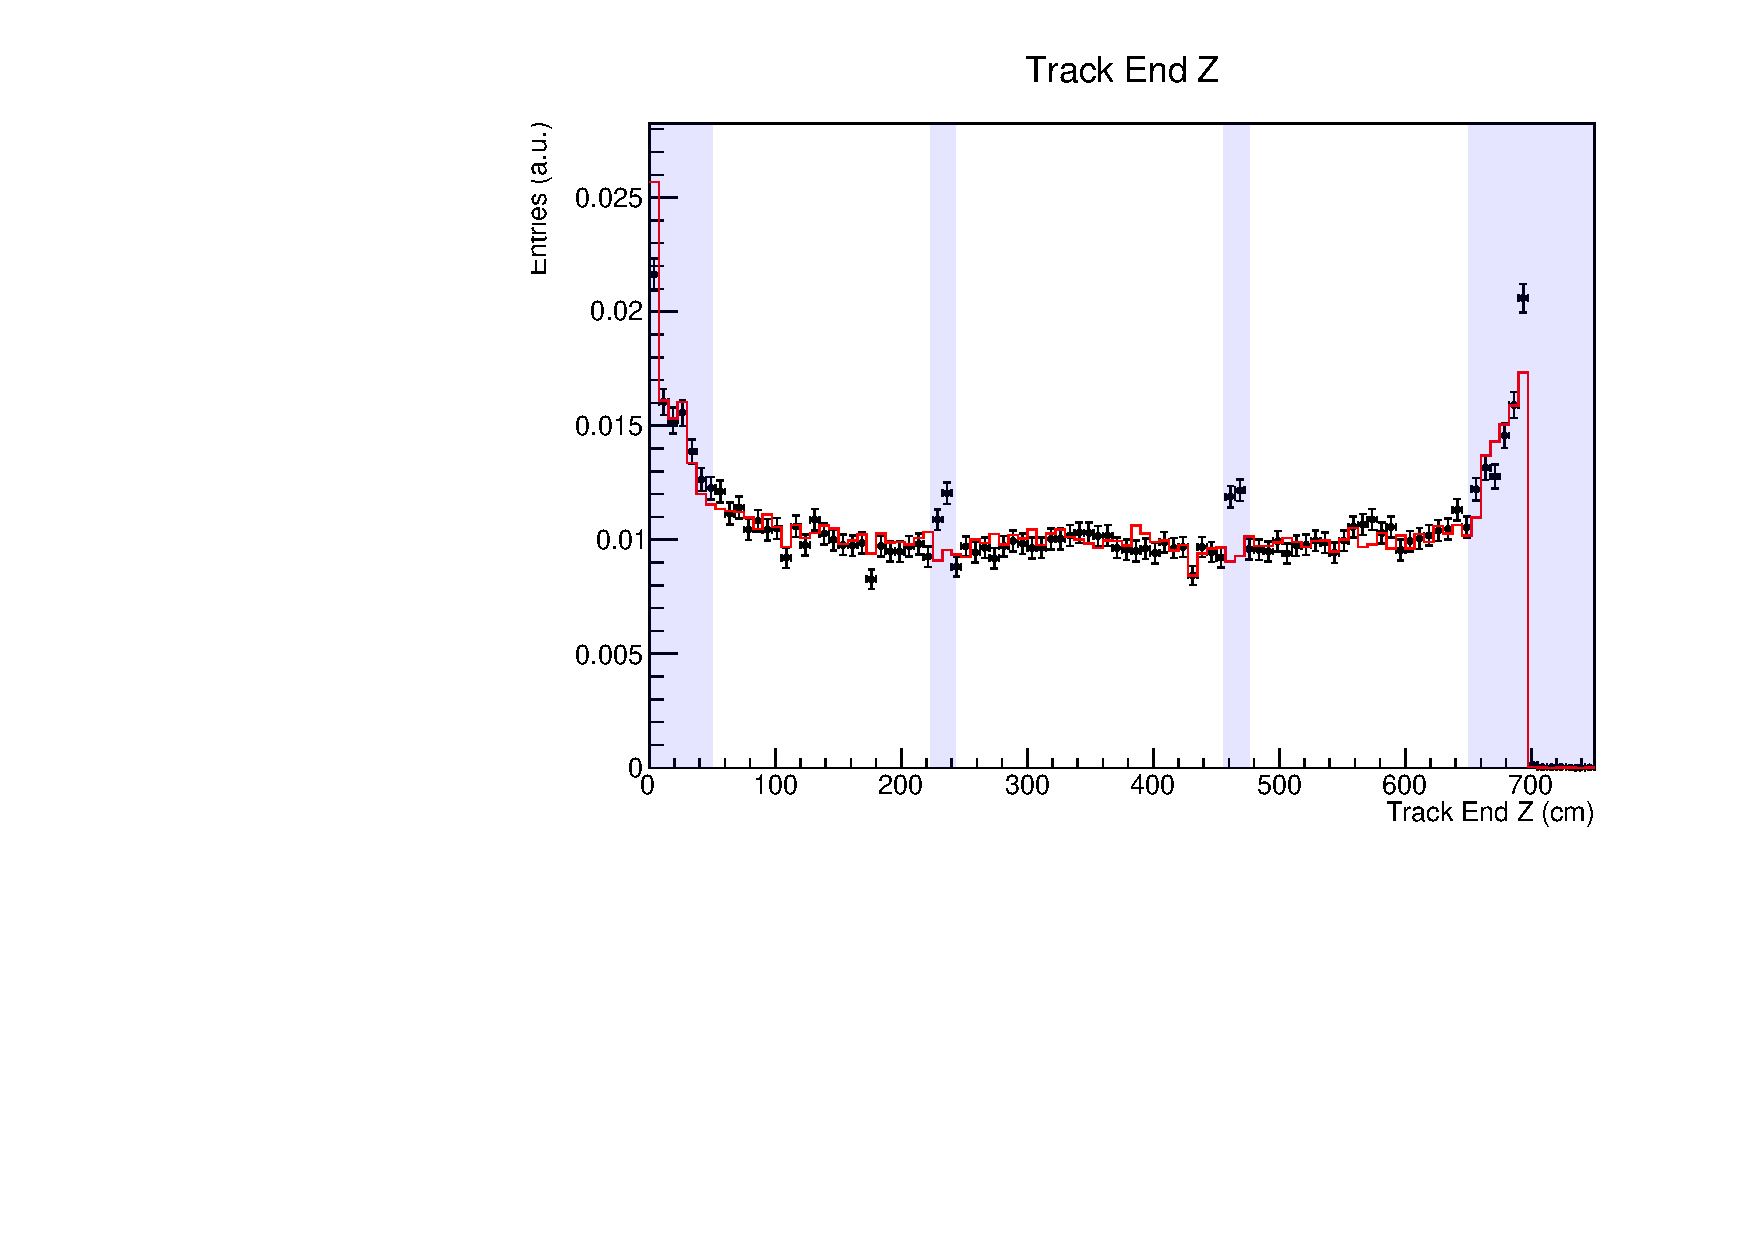
\includegraphics[width=0.49\textwidth]{figures/endZ_nocuts.pdf}
		\caption {An example of spatial cuts applied to the X, Y, and Z coordinates
		of the track endpoint.}
		\label{fig:spatial_cuts}
	\end{subfigure}
	\begin{subfigure}[b]{\textwidth}
		\centering
		\vspace{1.5cm}
		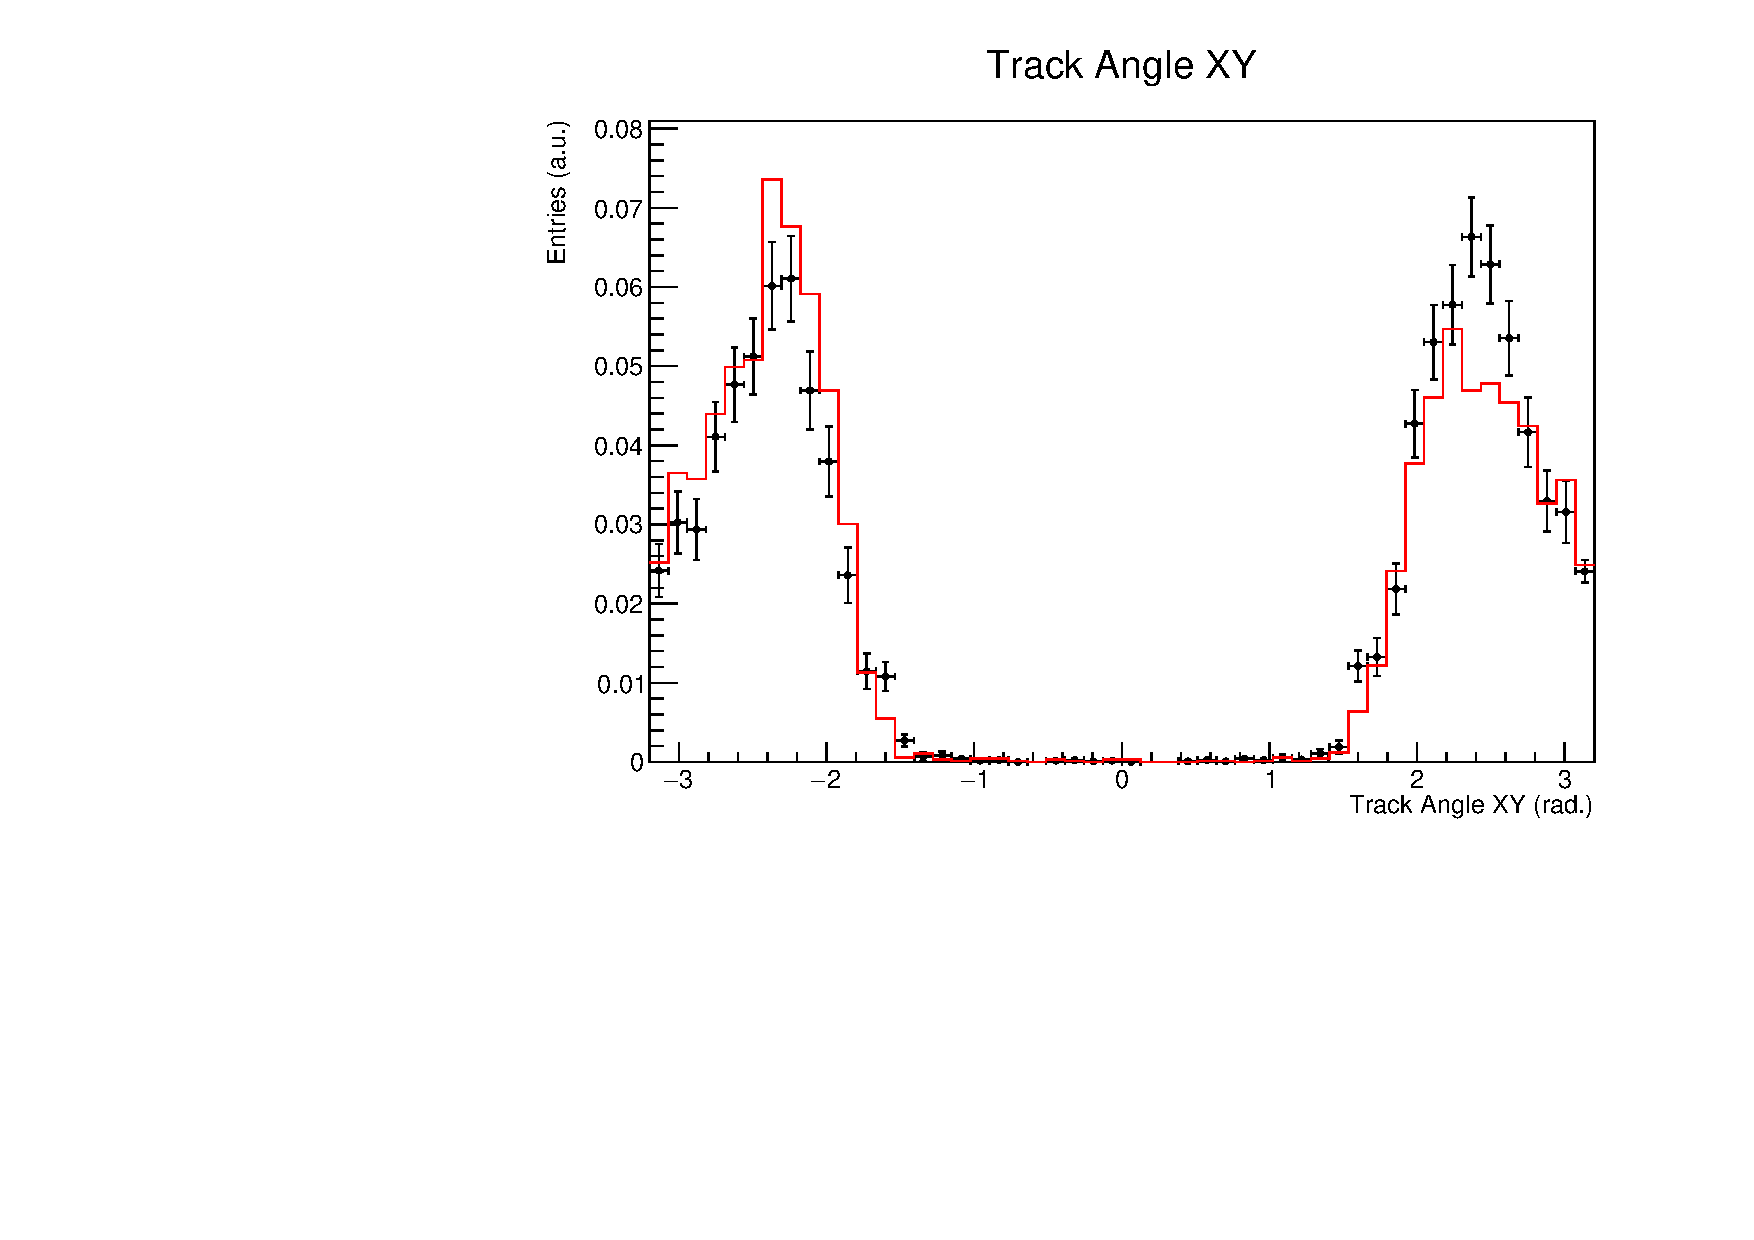
\includegraphics[width=0.49\textwidth]{figures/angXY_cuts.pdf}
		\hfill
		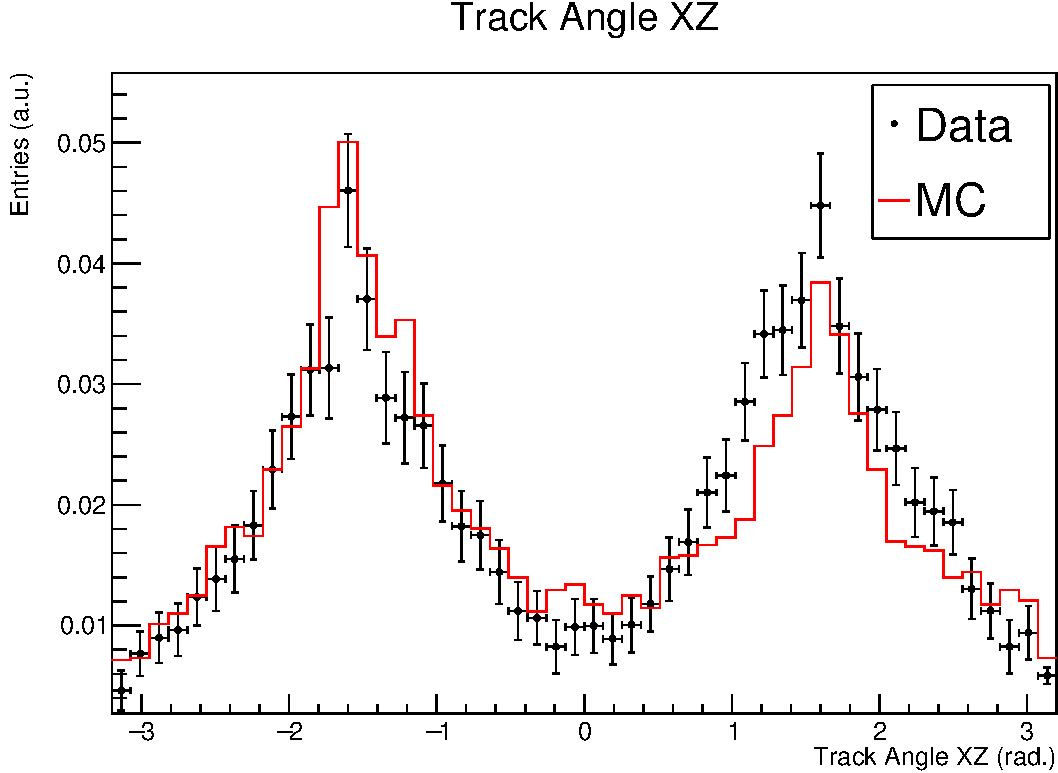
\includegraphics[width=0.49\textwidth]{figures/angXZ_cuts.pdf}
		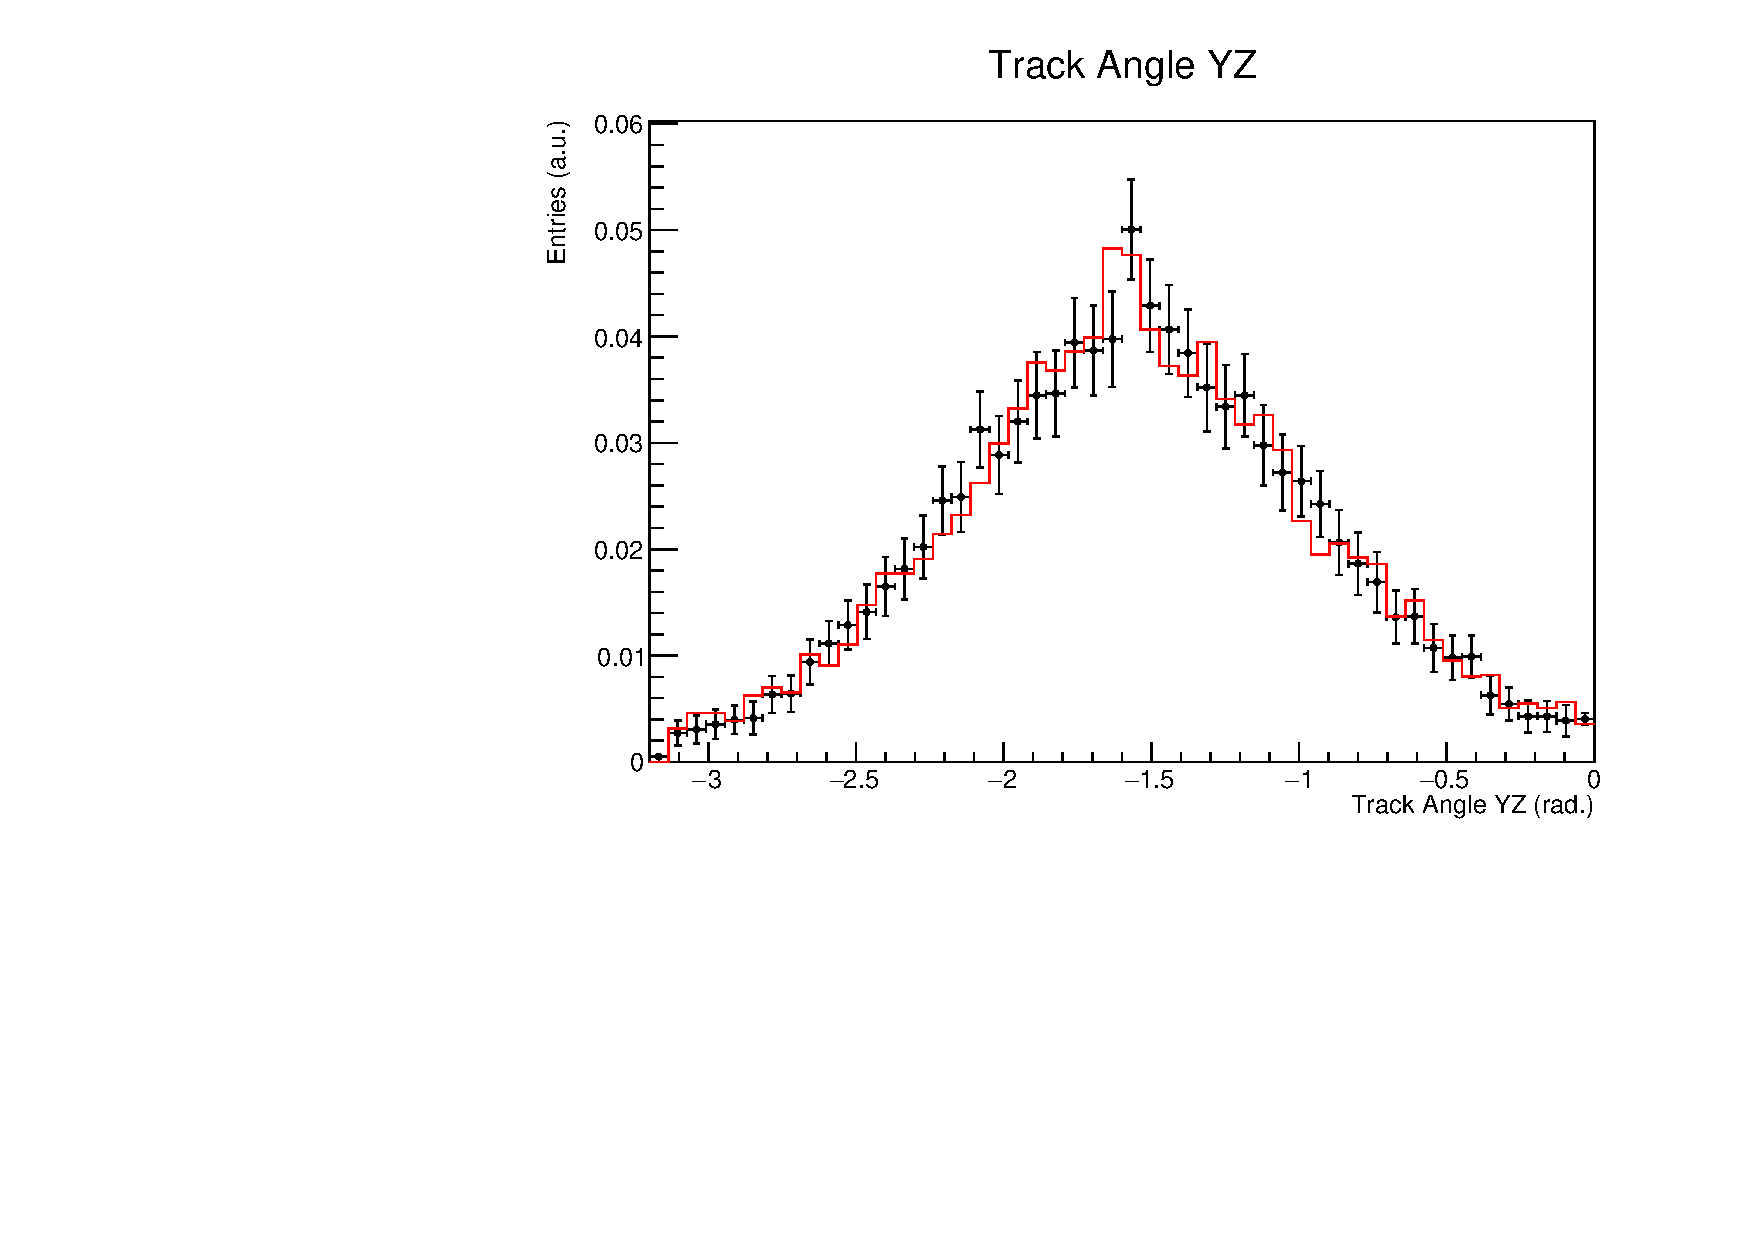
\includegraphics[width=0.49\textwidth]{figures/angYZ_cuts.pdf}
		\caption {Track angular distributions after spatial cuts in 
		\subref{fig:spatial_cuts} applied.}
		\label{fig:angular_dist}
	\end{subfigure}

	\caption 
	[Data Quality Cuts for CNN Comparison.]
	{Data Quality Cuts for CNN Comparison.}
	\label{fig:cnn_cuts_spatial}

\end{figure}

The shower classifier scores for the pion, proton, and electron test beam 
samples are shown in Figure \ref{fig:cnn_scores_beam}. The data in the pion 
and proton distributions was taken from \protodune{} run 5387, and the data in 
the electron distribution was from run 5809. The data in all of these beam
particle distributions are normalised by the number of triggered 
beam particles of the given flavour.
\begin{figure}

	\centering

	\begin{subfigure}[b]{0.68\textwidth}
		\centering
		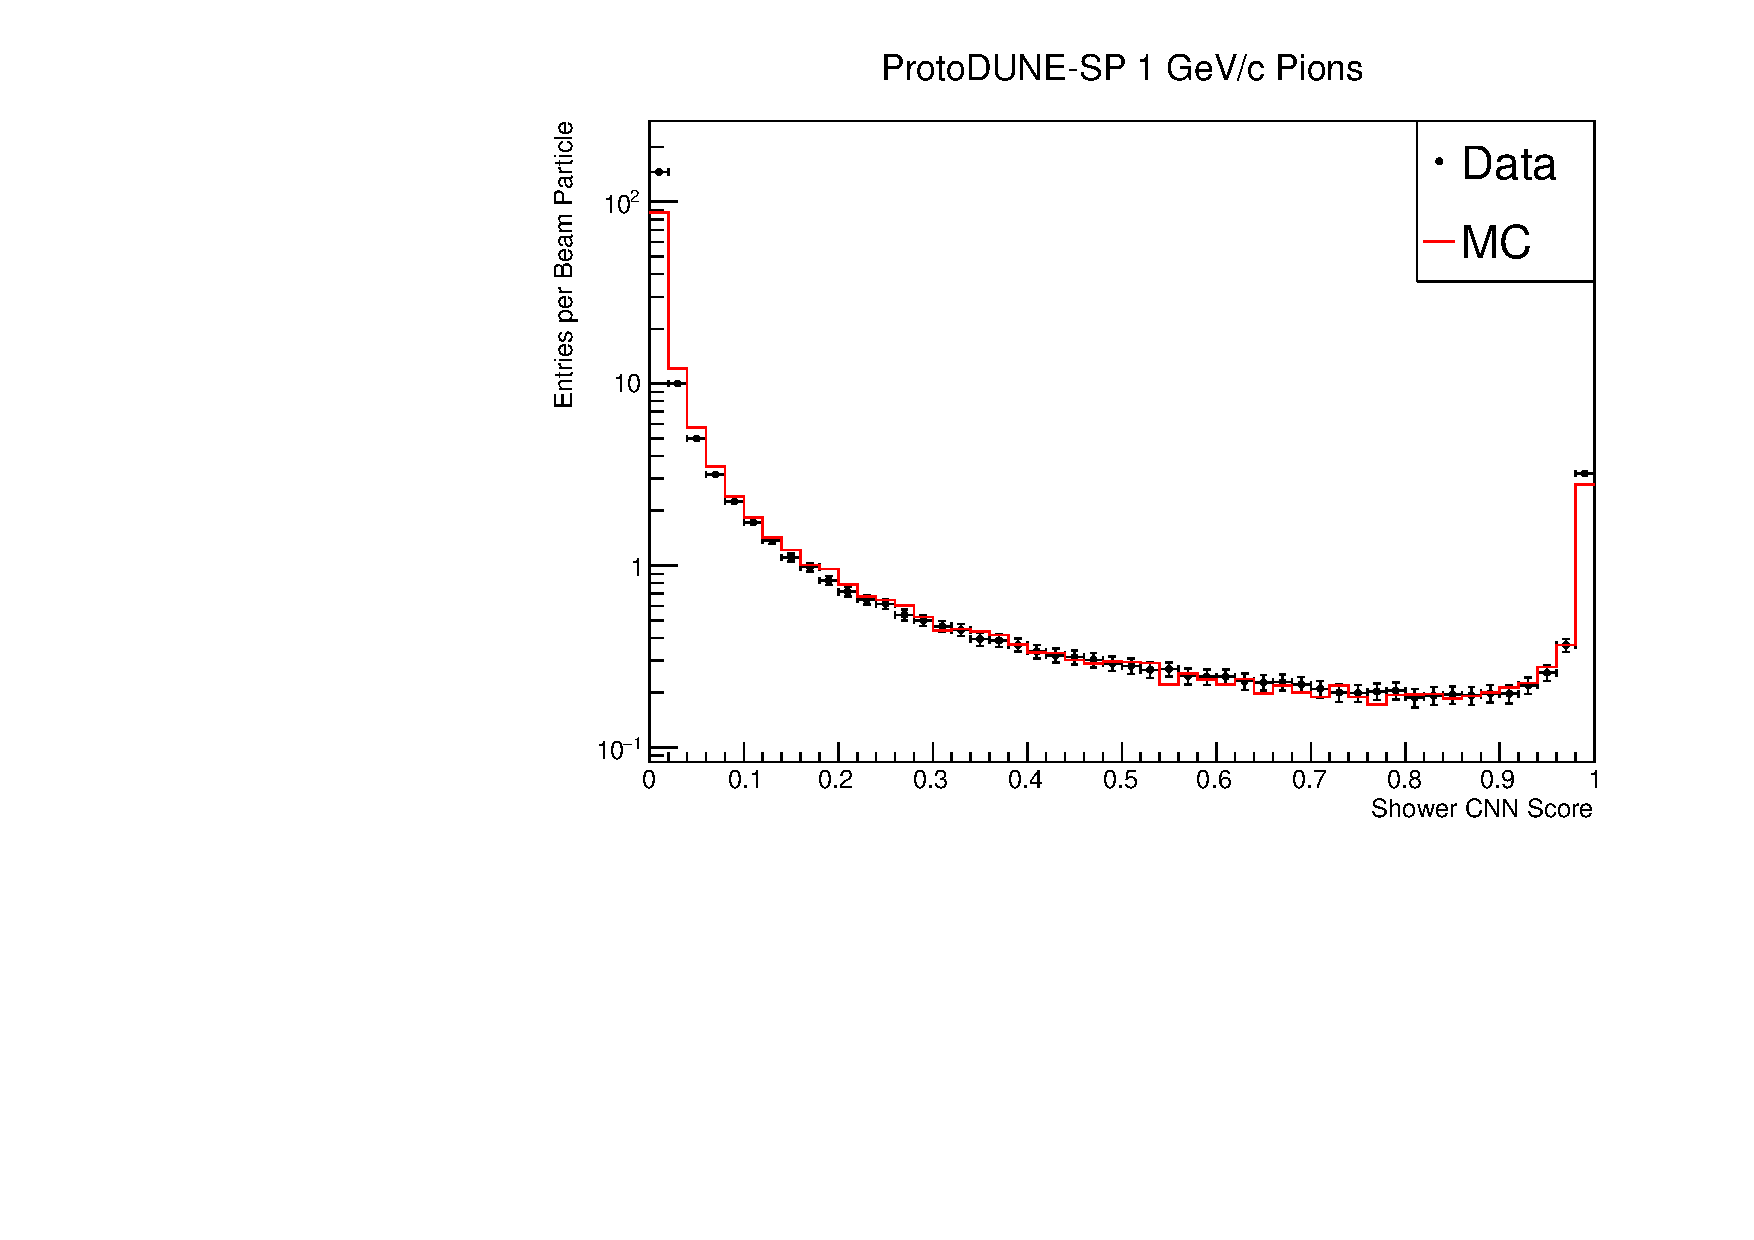
\includegraphics[width=\textwidth]{figures/hit_cnn_pion.pdf}
		\caption {Pions.}
		\label{fig:beam_pi_cnn}
	\end{subfigure}

	\begin{subfigure}[b]{0.68\textwidth}
		\centering
		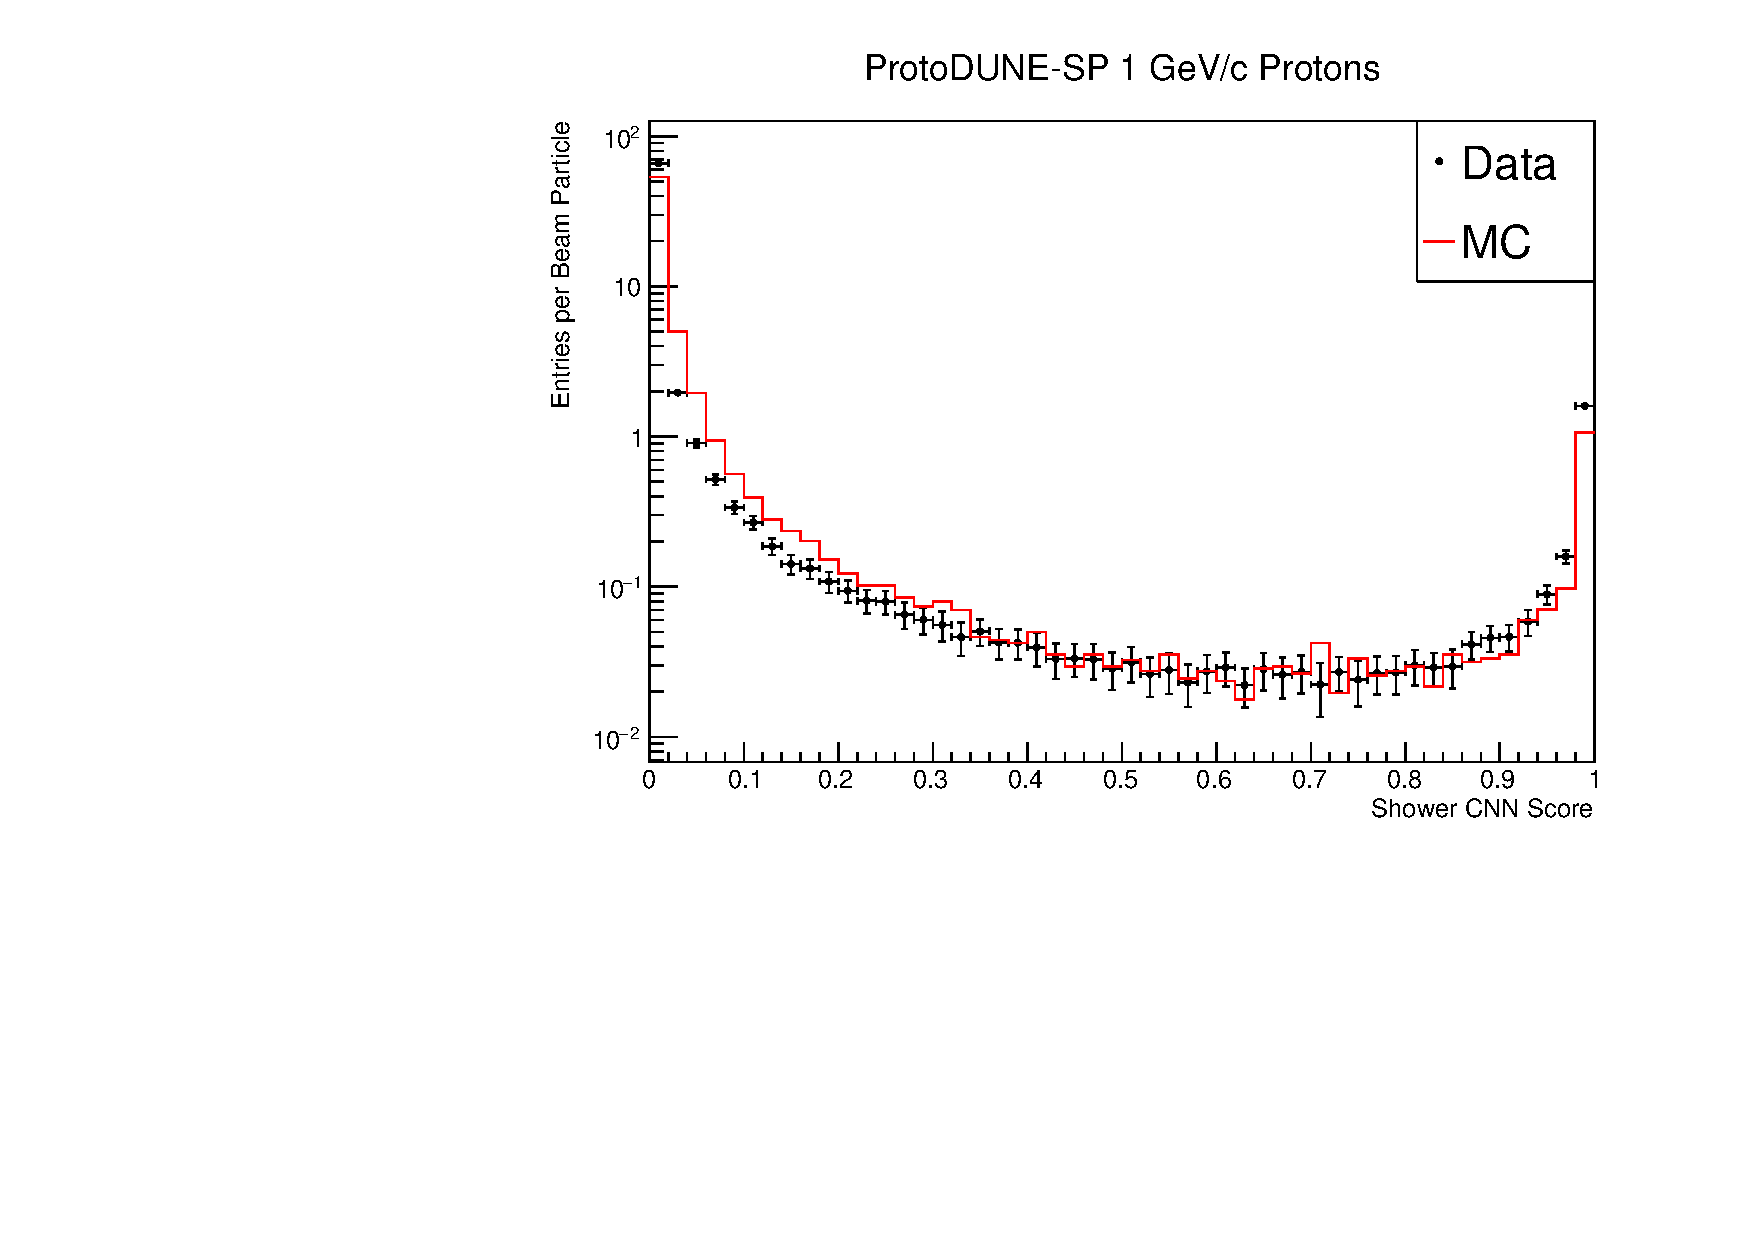
\includegraphics[width=\textwidth]{figures/hit_cnn_proton.pdf}
		\caption {Protons.}
		\label{fig:beam_proton_cnn}
	\end{subfigure}

	\begin{subfigure}[b]{0.68\textwidth}
		\centering
		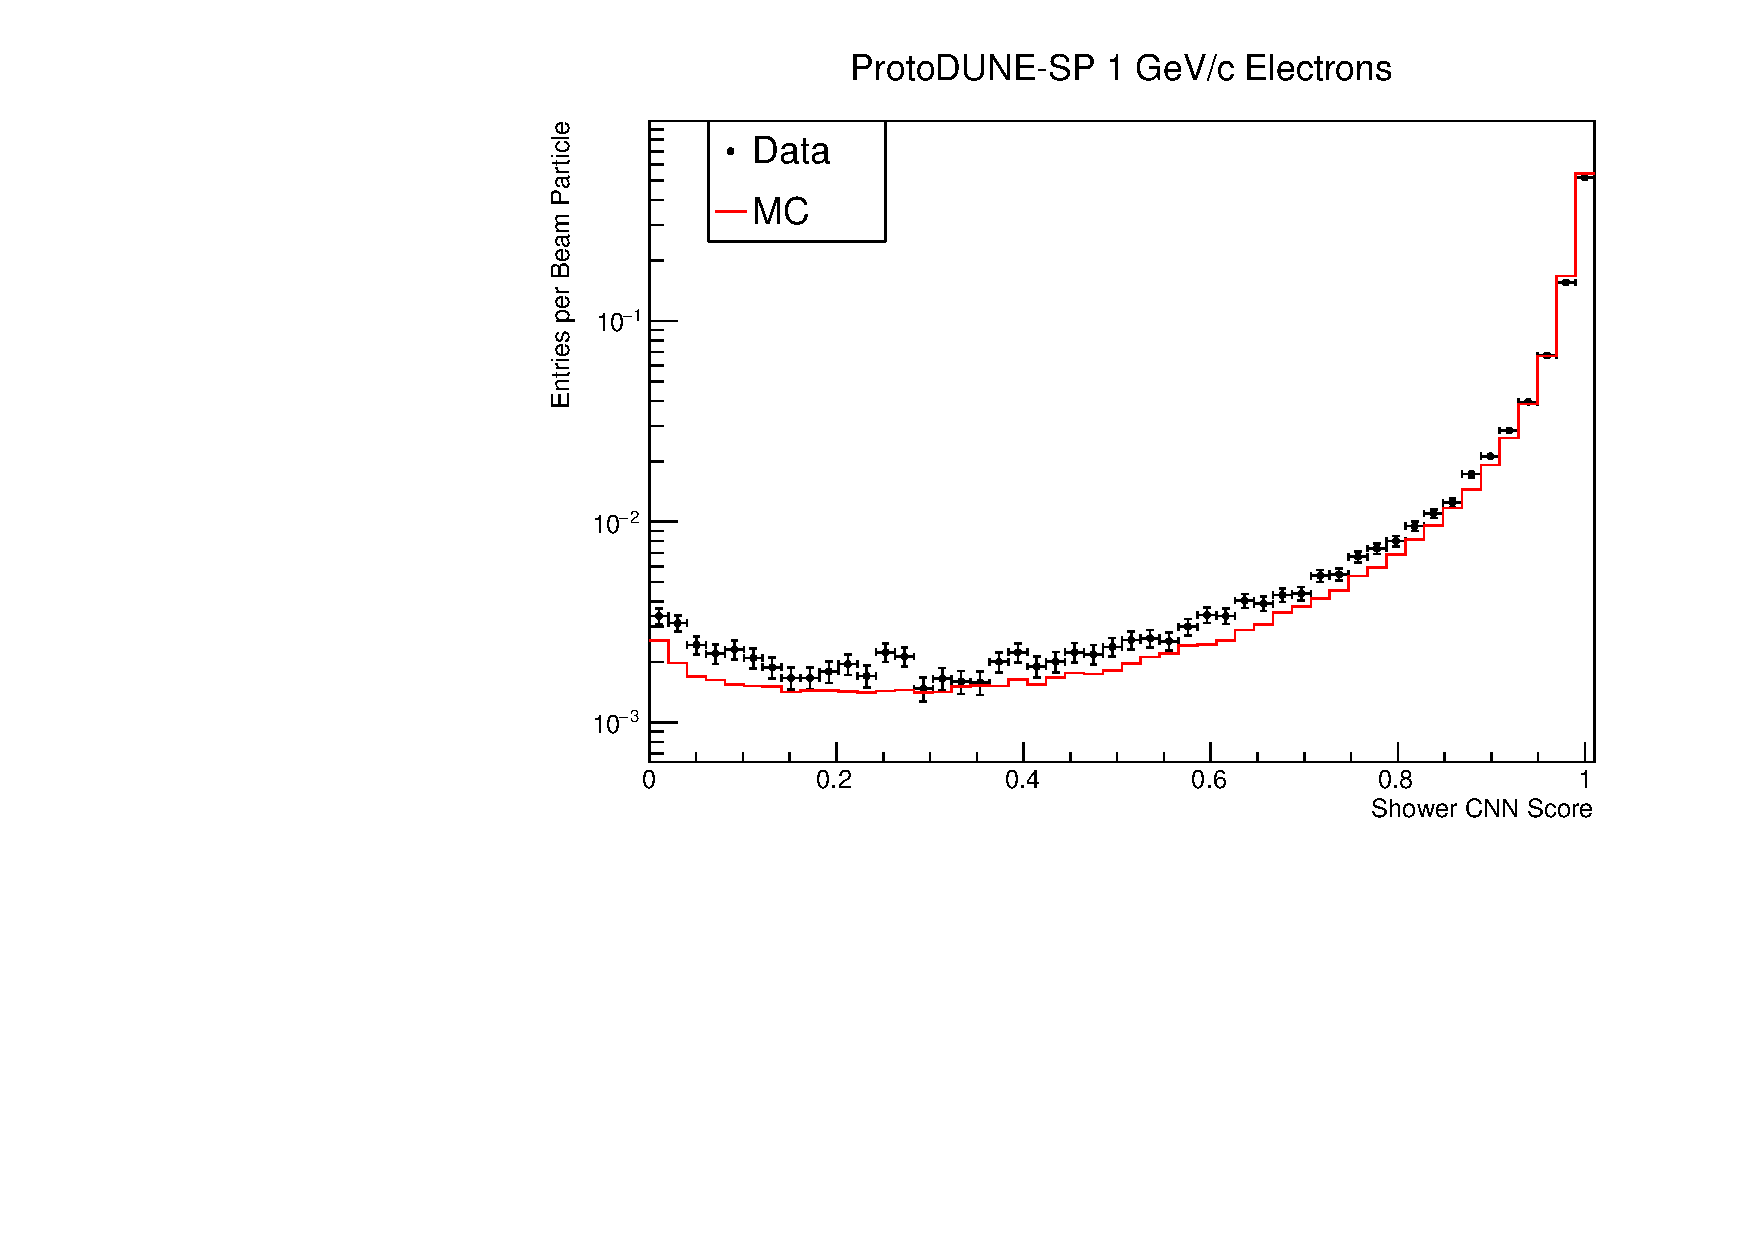
\includegraphics[width=\textwidth]{figures/hit_cnn_electron.pdf}
		\caption {Electrons.}
		\label{fig:beam_electron_cnn}
	\end{subfigure}

	\caption
	[Shower classifier scores for different particle species from the \protodune{} 
	beam.]
	{Shower classifier scores for different particle species from the \protodune{} 
	beam, in data and simulation.}
	\label{fig:cnn_scores_beam}

\end{figure}

Overall, there is a good agreement between the data and simulation in terms of
the shower score distributions for each particle species. However, there are
still some discrepancies, which highlights the differences between the data and
the simulation. The difference is most pronounced for the electron sample, which
gets consistently more entries at low CNN scores. One consistent difference
between data and simulation for all particle species, is the tendency for 
Pandora to cluster more hits into each reconstructed particle in data than in 
simulation. This can be seen in the bins at the two ends of the distributions,
which contain the majority of the hits, and consistently have more entries in 
data than in simulation.

The cosmic--ray sample was selected based on the cosmic--ray part of the
Pandora reconstruction chain, discussed in Chapter \ref{ch:protodune}. Any
reconstructed particles, which have been labelled as both clear cosmic--rays
and tracks by Pandora are included in the sample. The data in this sample was
taken from run 5387; while a cosmic--ray only run would be preferable, all of 
the \protodune{} simulations include test beam particles. Therefore, a test beam
run was chosen in order to match as closely as possible to the simulation.

The shower score distribution for cosmic--ray tracks is shown in Figure
\ref{fig:cosmic_muon_cnn}. These distributions are normalised by the total
number of hits in each distribution, this is because there is a large difference
in the average number of reconstructed hits in clear cosmic--rays from Pandora
between data and simulation. Again a good agreement is seen over the majority 
of the range, but in data there is a prominent excess of hits with a high 
shower score. The cause of this excess is not currently understood, one
possibility is that delta--rays are more often reconstructed as part of
cosmic--ray tracks in data than in simulation.

\begin{figure}
	\centering
	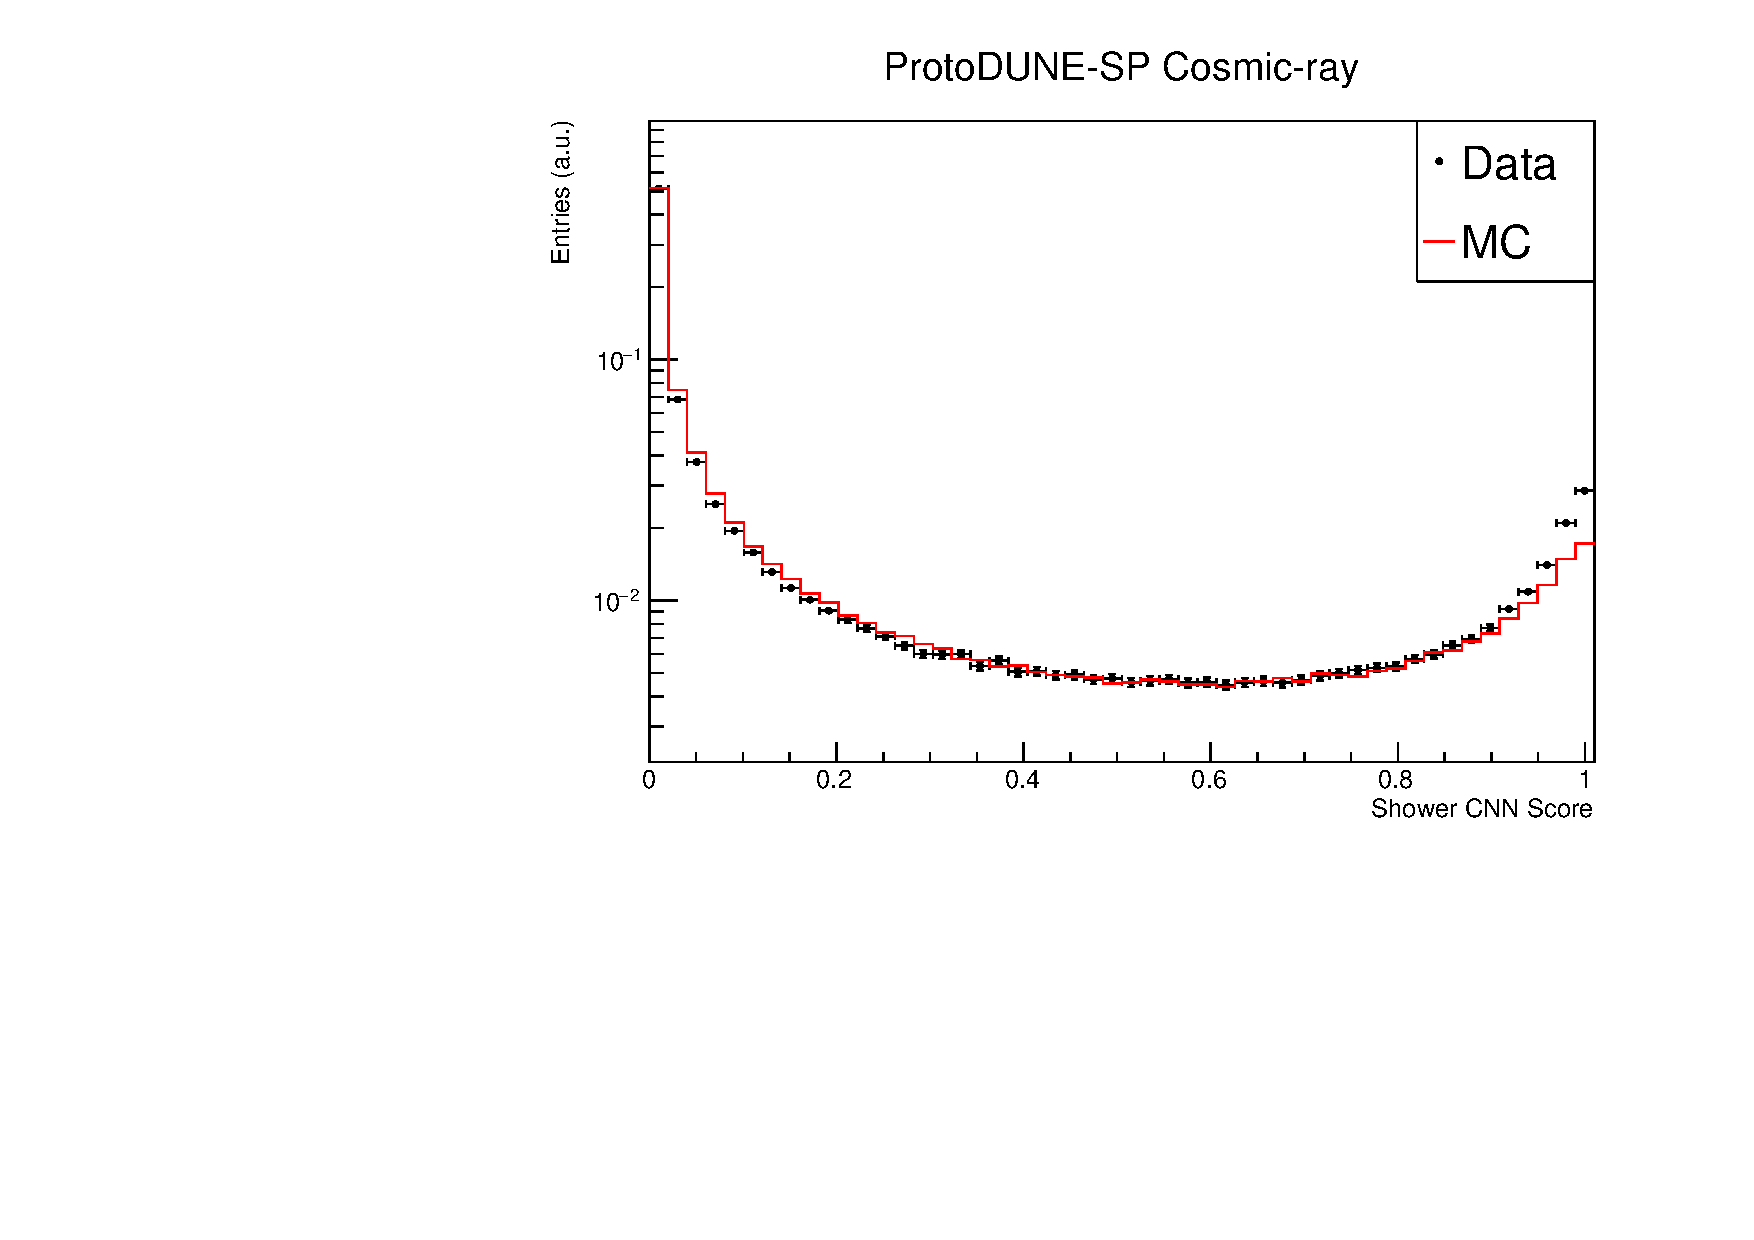
\includegraphics[width=\textwidth]{figures/hit_cnn_cosmics.pdf}
	\caption
	[Shower classifier score for hits from cosmic--rays.]
	{Shower classifier score for hits from reconstructed cosmic--rays, in data and
	simulation.}
	\label{fig:cosmic_muon_cnn}
\end{figure}

\bigskip
\noindent
In practice, the CNN will be used to select events based on choosing hits with 
CNN scores above some threshold. This could be based on an average over a 
number of hits, on a hit by hit basis, or something more complicated. For the
purposes of understanding the approximate errors involved in selecting hits with
the CNN, we will consider selecting hits on a hit--by--hit basis here.  The 
uncertainties involved with selecting hits in this way can be evaluated by 
considering the fraction of hits selected into the sample given a selection 
threshold. 

In Table \ref{tab:frac_selected}, we list the fraction of individual hits 
selected into the appropriate category for each sample in data and simulation. 
The fractional difference between the numbers in each case is an estimate of 
the percentage uncertainty associated with this simple selection algorithm. 
For the sample of all hits, the track category was used, and a fractional
difference of 1\% was seen. This varies depending on the particle species, 
with the largest difference being 3\% for the cosmic--ray sample. 
\begin{table}
	\centering
	\bgroup 
	\def\arraystretch{1.5}
	\begin{tabularx}{\textwidth}{@{}c|c|Y|Y|c@{}}
		Hit Source  & Class  & MC Fraction (\%) & Data Fraction (\%) & Data / MC\\\hline
		All         & Track  & 77.1             & 76.2               & 0.99     \\
		Pion        & Track  & 93.8             & 95.4               & 1.02     \\
		Proton      & Track  & 97.1             & 96.6               & 0.99     \\
		Electron    & Shower & 96.9             & 95.8               & 0.99     \\
		Cosmic--ray & Track  & 92.9             & 90.3               & 0.97
	\end{tabularx}
	\egroup
	\caption
	[Fraction of hits in correct class for different samples in \protodune{} data 
	and simulation.] 
	{Fraction of hits in correct class for different samples in \protodune{} data 
	and simulation.}
	\label{tab:frac_selected}
\end{table}

Overall, the CNN results have been shown to agree well with data across a 
range of particle types. The discrepancies seen are also influenced by the 
difference between data and simulation for the Pandora reconstruction 
framework, which makes the cause of the discrepancies difficult to 
disentangle. However, the general agreement between data and simulation is a 
sign that the results from the CNN are sensible, and the additional 
classification strength of the CNN over Pandora makes it a useful tool in 
analyses of the \protodune{} data. The discrepancies will impact each analysis 
differently, therefore, the uncertainties involved with using the CNN 
classifier should evaluated on a case--by--case basis; for hit selection with 
a simple hit--by--hit algorithm the uncertainties are on the order of 1-3\%
depending on the particle species.

\section{Application in \protodune{} Analyses} \label{cnn-appl}
The output of the CNN classifier has been applied in a number of \protodune{}
analyses since it was developed. Chapter \ref{ch:michel} will detail one use of
the network in a Michel electron analysis. In addition, the scores from the
network are being incorporated into analyses by other members of the 
\protodune{} experiment, including:
\begin{itemize}
	\item Selecting shower candidates for neutral--pion event selection\cite{pi_0}.
	\item Identifying charge exchange candidates in charged--pion cross section 
		analyses\cite{pion_exchange}.
	\item Identifying Michel electron contaminated tracks for stopping muon
		calibration\cite{fabio_muon}.
\end{itemize}
